\chapter{Differential cross-section calculation}

\label{ch:analysis1D}
\vspace{-10pt}
This chapter delineates the specific steps I performed to extract the cross-section for MINERvA's first measurement of nuclear dependence in inclusive antineutrino scattering in medium energy. The analysis utilises data from an exposure of $1.12 \times 10^{21}$ protons on target (POT), and the simulation sample detailed in Chapter~\ref{ch:dataAsimulation}. Both the data and simulation were reconstructed using the techniques described in Chapter~\ref{ch:Reconstruction}. The differential cross-sections for carbon, hydrocarbon (scintillator), iron, and lead were determined using Equation~\ref{eq:xsec1D} for muon transverse momentum $p_{\text{T}}$ and Bjorken $x$. Additionally, the nuclear target to scintillator cross-section ratios were calculated using the matching flux technique discussed in Section~\ref{sec:nuclear_target_flux}. The results of this analysis are shown and discussed in Chapter~\ref{ch:results}, with the systematic uncertainties detailed in Chapter~\ref{ch:systematics}.

\iffalse
\fi
\section{Event selection}
\label{sec:eventSelection}

Event selection refers to a process of counting the number of interactions passing a set of selection cuts according to the analysis signal definition while taking into account the reconstruction capabilities of the detector. In this case, it ensures the cross-section is extracted for the charged-current interaction type inclusive sample of antineutrino scattering in a specific material. It is the first step of the cross-section extraction represented by $N_{\text{data}, j}$ in the Equation~\ref{eq:xsec1D} in Chapter~\ref{ch:measurement}.

The events considered in this analysis must meet the following criteria:
\begin{itemize}
    \item Charged-current antineutrino interaction producing an antimuon $\mu^{+}$
    \item Interaction occurring in a specific material, i.e. carbon, hydrocarbon iron, or lead
    \item Antimuon energy between 2 and 20 GeV
    \item Antimuon angle less than 17$^\circ$ with respect to the beam direction
\end{itemize}
The phase-space cuts included in the signal definition are determined by the detector's ability to reconstruct the antimuon, as discussed later.~It is also important to note that these selection criteria were also employed to compare the cross-section results with the corresponding samples from different (anti)neutrino event generators in Chapter~\ref{ch:results}.

Utilising the reconstructed data and the simulation sample from Chapter~\ref{ch:Reconstruction}, which comprises all MINERvA reconstructable MINOS-matched events, the same set of reconstruction cuts was applied to both samples. These cuts were aimed at identifying events that match the signal definition mentioned above, based on their reconstructed properties. Additionally, the reconstruction cuts serve to eliminate background events (i.e. non-signal events) and aid in the selection of events whose kinematics can be reconstructed while minimizing systematic uncertainties arising from the detector's reconstruction capabilities, as well as flux and interaction modelling. Most of these reconstruction cuts are shared across all MINERvA analyses as they stem from the MINERvA detector and the MINOS spectrometer designs. 

\begin{table}[b!]
    \centering

    \begin{tabular}{c c c c}
    \hline \\ [-1.5 ex]
    Target & Material & Number of events in data & Predicted purity (\%) \\ [0.5ex] % inserts table %heading
    \hline
    \hline
    2 & Iron & 75 786 & 84.4 \\
      & Lead & 68 559 & 86.4 \\
    \hline
    3 & Carbon & 56 760 & 81.7 \\
      & Iron & 36 647 & 84.0 \\
      & Lead & 22 809 & 87.0 \\
    \hline
    4 & Lead & 65 469 & 75.9 \\
    \hline
    5 & Iron & 52 247 & 78.7\\
      & Lead & 35 068 & 81.6 \\
    \hline
    Tracker & Scintillator & 1 823 367 & 98.9 \\
    \hline
    \end{tabular}

    \caption{Number of antineutrino data events reconstructed and selected in all relevant targets of different materials and the scintillator tracker of the MINERvA detector, and the predicted purity of the selection based on the simulation.}
    \label{table:selectedEvents}
\end{table}


Furthermore, although the final cross-section results are reported for various materials, most of the analysis steps treat individual targets of different materials separately. This separation is necessitated by the distinct efficiencies of the various target and material combinations discussed later on in Section~\ref{ch:efficiency}, which result from their positions in the detector. Therefore, this is also taken into account in the list of reconstruction cuts, which is as follows:
\begin{enumerate}
    \item The antimuon detected in the MINOS spectrometer must have a positive curvature to ensure an $\bar{\nu}_{\mu}$ interaction occurred, i.e. $(q/p) > 0$, where $q$ is the antimuon's charge and $p$ its momentum.
    \item The high-energy antimuon reconstructed by curvature in the MINOS spectrometer must have a curvature significance at least 5$\sigma$ to reduce the tails of the muon energy resolution spread \cite{Joel_HighMomMuons}, i.e. $(q/p)/\sigma_{q/p} \geq 5$, where $\sigma_{q/p}$ is the error on the curvature.
    % this  (q\p)/sigma (sigma is the error on q\p)
    \item The antimuon track must be contained within the fiducial volume of the MINOS spectrometer and cannot cross MINOS coil hole described in Chapter~\ref{ch:minerva}, i.e.~the event track must fall within the radial distance of \mbox{$210~\text{mm} < R_{\text{event}} < 2500~\text{mm}$ \cite{Joel_HighMomMuons, MINOS:1998kez}.}
    % https://minerva-docdb.fnal.gov/cgi-bin/sso/ShowDocument?docid=10154
    \item The interaction vertex must be within the fiducial volume of the MINERvA detector. This is bounded by a hexagon with an $850$ mm apothem in the $x$-$y$ plane, and for mixed targets, the vertex must be located more than $25~\text{mm}$ away from the boundary between the different materials \cite{Aliaga_2014}.
    \item The event must not contain any dead channels, i.e.~channels insensitive to new energy deposits, induced by previous interactions in the path projected upstream of the muon track. This is to avoid rock muons whose tracks are partially lost due to the dead time from being confused with fiducial events \cite{Aliaga_2014}.
    % https://www.sciencedirect.com/science/article/pii/S0168900214000035
    \item The event is excluded if the highest machine-learning probability for vertex placement falls below 20\% to eliminate instances where the network may be uncertain, maintaining a consistent and statistically significant contribution with similar pass rates for both data and simulation \cite{Klustova_MLsys}.
    % https://minerva-docdb.fnal.gov/cgi-bin/sso/ShowDocument?docid=29420
    \item For hydrocarbon (scintillator), the $z$ position of the machine-learning (ML) vertex must be in the tracker region, i.e. $5980~\text{cm} \geq z \geq 8422~\text{cm}$. For carbon, iron, and lead, the $z$ position of the interaction vertex must be located within the passive target 2, 3, 4, or 5 as described in Chapter~\ref{ch:Reconstruction}, and in the region of the $x$-$y$~plane corresponding to the respective material as discussed in Chapter~\ref{ch:minerva}. Target 1 is excluded from this analysis due to contamination from rock muons. As the most upstream target, it has only a small number of upstream tracking planes, making it challenging to distinguish an interaction in this target from a rock muon solely based on the antimuon track.
    % ML vertexing https://minerva-docdb.fnal.gov/cgi-bin/sso/ShowDocument?docid=16995
    \item The energy of the antimuon must be within the range of 2 to 20 GeV. The lower limit ensures that the antimuon possesses enough energy to traverse through the MINERvA detector and cross multiple planes in the MINOS spectrometer to form a track. Meanwhile, the upper limit serves to minimize neutrino contamination in the sample, particularly from unfocused high-energy mesons that have not undergone charge selection. Crucially, the 20 GeV cut-off is imposed due to an incomplete understanding of the flux modelling beyond this threshold.
    % cite Brian? 
    \item The angle of the antimuon with respect to the antineutrino beam must be less than~17$^\circ$.~This requirement is driven by the steep decline in the acceptance of the MINOS spectrometer for larger scattering angles, especially for interactions occurring in the most upstream nuclear targets. This is demonstrated in the $p_{\text{T}}$ efficiency plots, where $p_{\text{T}}$ serves as a direct proxy for the antimuon angle, later on in Section~\ref{ch:efficiency}.   
\end{enumerate}
Included in Appendix~\ref{ch:appendix_eventSelection} is an illustrative comparison showcasing the impact of each of these cuts on target 5 lead and the scintillator tracker in both data and simulation.

\iffalse
Target 5 Lead Data vs MC
MINOS matched events:
Antimuon:
5 sigma:
MINOS fiducial:
MINERvA fiducial:
Dead channels:
ML probability:
Tracker or Target + material:
Energy:
Angle:
\fi

The number of antineutrino events reconstructed and selected in all relevant targets of different materials and the scintillator tracker of the MINERvA detector is listed in Table~\ref{table:selectedEvents}.~In total, this measurement utilises an extensive dataset of antineutrino interactions: 56 760 in carbon, 164 680 in iron, \mbox{191 905} in lead, and 1 823 367 in hydrocarbon (scintillator tracker).~For comparison, this represents approximately $10\times$~more statistics than those in the MINERvA neutrino analysis in nuclear targets in low energy \cite{Tice_PhysRevLett.112.231801}, as mentioned in Section~\ref{ch:measurement}. Most importantly, it constitutes the largest sample of antineutrino interactions on various materials in the same beam ever analysed to date. 

\begin{figure}[t!] 
    \centering
    {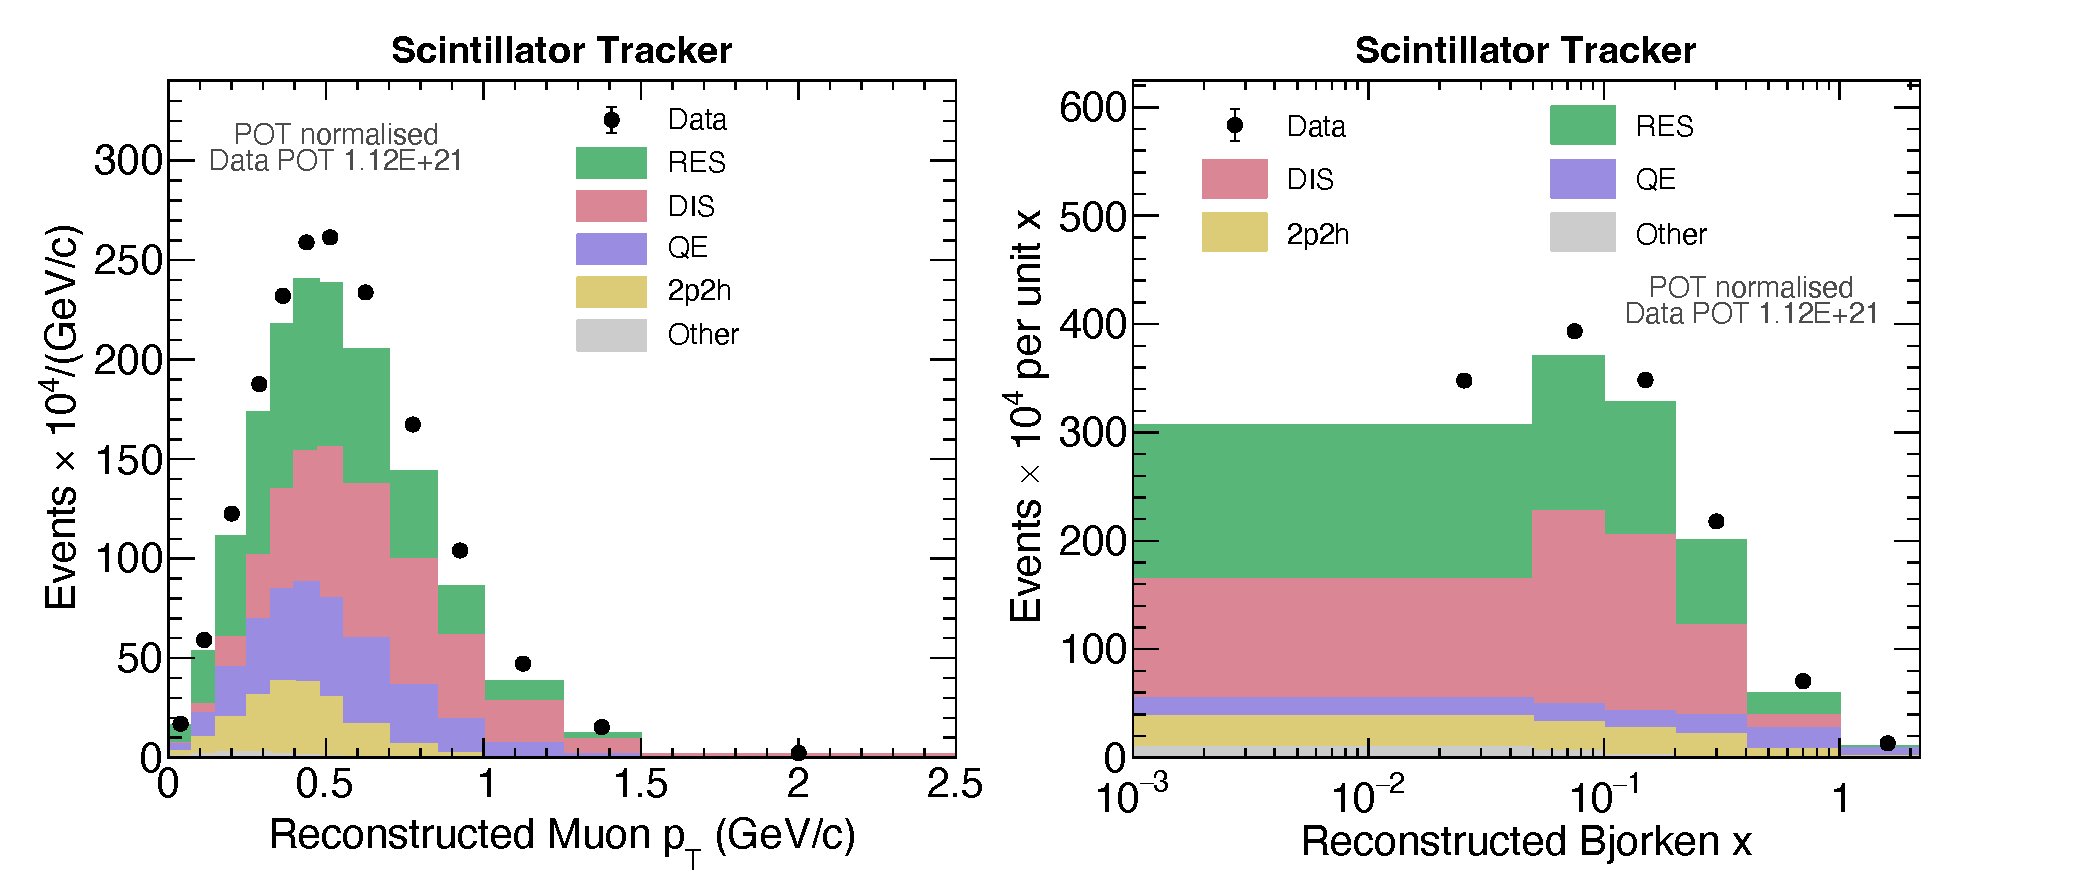
\includegraphics[width=1.\textwidth]{07analysis1D/figures/eventSelection_intType_tracker_pTx.pdf}}%
    \caption{Selected event distributions in the scintillator tracker for both antimuon $p_{\text{T}}$ (left) and Bjorken $x$ (right). The distributions are bin-width and POT normalised. The black points represent the data with its statistical uncertainty, while the simulation is broken down into the various interaction channels stacked in the descending order of their contribution:~resonant pion production (RES), deep inelastic scattering (DIS), quasi-elastic scattering (QE), 2p2h interaction (2p2h), and Other. The simulation visibly underpredicts the data in the scintillator tracker.}
    \label{fig:eventSelection_intType_tracker_pTx}
\end{figure}

Figure~\ref{fig:eventSelection_intType_tracker_pTx} displays the bin-width normalised distributions of selected events in the scintillator tracker for both variables of interest: muon $p_{\text{T}}$ and Bjorken $x$. Bin-width normalisation in this context means that each bin is divided by its own width. Therefore, the actual content of the bin is the number read off the $y$-axis (with $10^4$ included) multiplied by the bin width. The bin edges of antimuon $p_{\text{T}}$ and Bjorken $x$ are listed in Table~\ref{table:bindEdges}. The determination of bin edges involved optimizing the diagonal of a migration matrix explained in Section~\ref{sec:migration_unfolding}. This optimization aimed to retain the interesting $x > 1$ bin in the Bjorken $x$ distribution, as discussed in Chapter~\ref{ch:measurement}, while the lower bin boundary was approximately set using the definition of Bjorken $x$ in Chapter~\ref{ch:measurement} and the value of the lowest $p_{\text{T}}$ bin. Additionally, the $p_{\text{T}}$ distribution was truncated at 2.5 GeV/$c$ due to limitations of the MINOS acceptance, as demonstrated in the $p_{\text{T}}$ efficiency plots in Section~\ref{ch:efficiency}.

The simulation prediction for the scintillator tracker in Figure~\ref{fig:eventSelection_intType_tracker_pTx} is categorized by various interaction types. Given that this inclusive analysis utilises antineutrino data collected during the medium-energy (ME) physics runs of the MINERvA detector, where the antineutrino flux peaks near $6$ GeV, the predominant interaction types are resonant pion production and deep inelastic scattering.~Across all targets of various materials, resonant pion production contributes, on average, around 38\% to the sample, while deep inelastic scattering makes up about 32\%. Quasi-elastic scattering and 2p2h interaction constitute approximately 18\% and 11\% of the sample, respectively. Other interaction types, including coherent pion production and others, contribute less than 1\% combined. An example of the nuclear target 5 lead distribution with the simulation broken down into various interaction types is also included in Appendix~\ref{ch:appendix_eventSelection}.

\begin{table}[t!]
    \centering
    \small

    \begin{tabularx}{1\textwidth}{p{0.125\textwidth} p{0.028\textwidth} p{0.048\textwidth} p{0.038\textwidth} p{0.038\textwidth} p{0.046\textwidth} p{0.028\textwidth} p{0.046\textwidth} p{0.036\textwidth} p{0.028\textwidth} p{0.036\textwidth} p{0.026\textwidth} p{0.033\textwidth} p{0.026\textwidth} p{0.023\textwidth}}
    \hline \\ [-1.5 ex]
    Variable & \multicolumn{14}{c}{Bin edges} \\ [0.5ex] % inserts table %heading
    \hline
    \hline
    $p_{\text{T}}$ (GeV/$c$) & 0.0 & 0.075 & 0.15 & 0.25 & 0.325 & 0.4 & 0.475 & 0.55 & 0.7 & 0.85 & 1.0 & 1.25 & 1.5 & 2.5 \\
    \hline
    Bjorken $x$ & \multicolumn{2}{c}{0.001}  & \multicolumn{2}{c}{0.05}  & \multicolumn{2}{c}{0.1}  & \multicolumn{2}{c}{0.2}  & \multicolumn{2}{c}{0.4}  & \multicolumn{2}{c}{1.0}  & \multicolumn{2}{c}{2.2}  \\
    \hline
    \end{tabularx}
    \caption{Bin edges of the antimuon $p_{\text{T}}$ and Bjorken $x$ histograms used in this analysis.}
    \label{table:bindEdges}
\end{table}

The aforementioned reconstruction cuts may not exclusively isolate signal events, leading to a contamination of the data sample by background events—--interactions that exhibit a similar signature to signal events in the detector and are misidentified as such. To estimate the level of contamination in the reconstructed data sample, the simulation with known true information can be utilised. The metric that does that is called predicted purity, defined as
\begin{equation}
    \label{eq:purity}
    %\vspace{-10pt}
    \text{Purity} = \frac{\text{Signal events in the reconstructed sample}}{\text{All events in the reconstructed sample}} \hspace{5pt}.
\end{equation}
The analysis predicted purity for all relevant targets of different materials and the scintillator tracker of the MINERvA detector is listed in Table~\ref{table:selectedEvents}. The nuclear target purity averages around 82\%, while the scintillator tracker purity is almost 99\%. 
% target average: 82.4625

\begin{figure}
    \centering
    {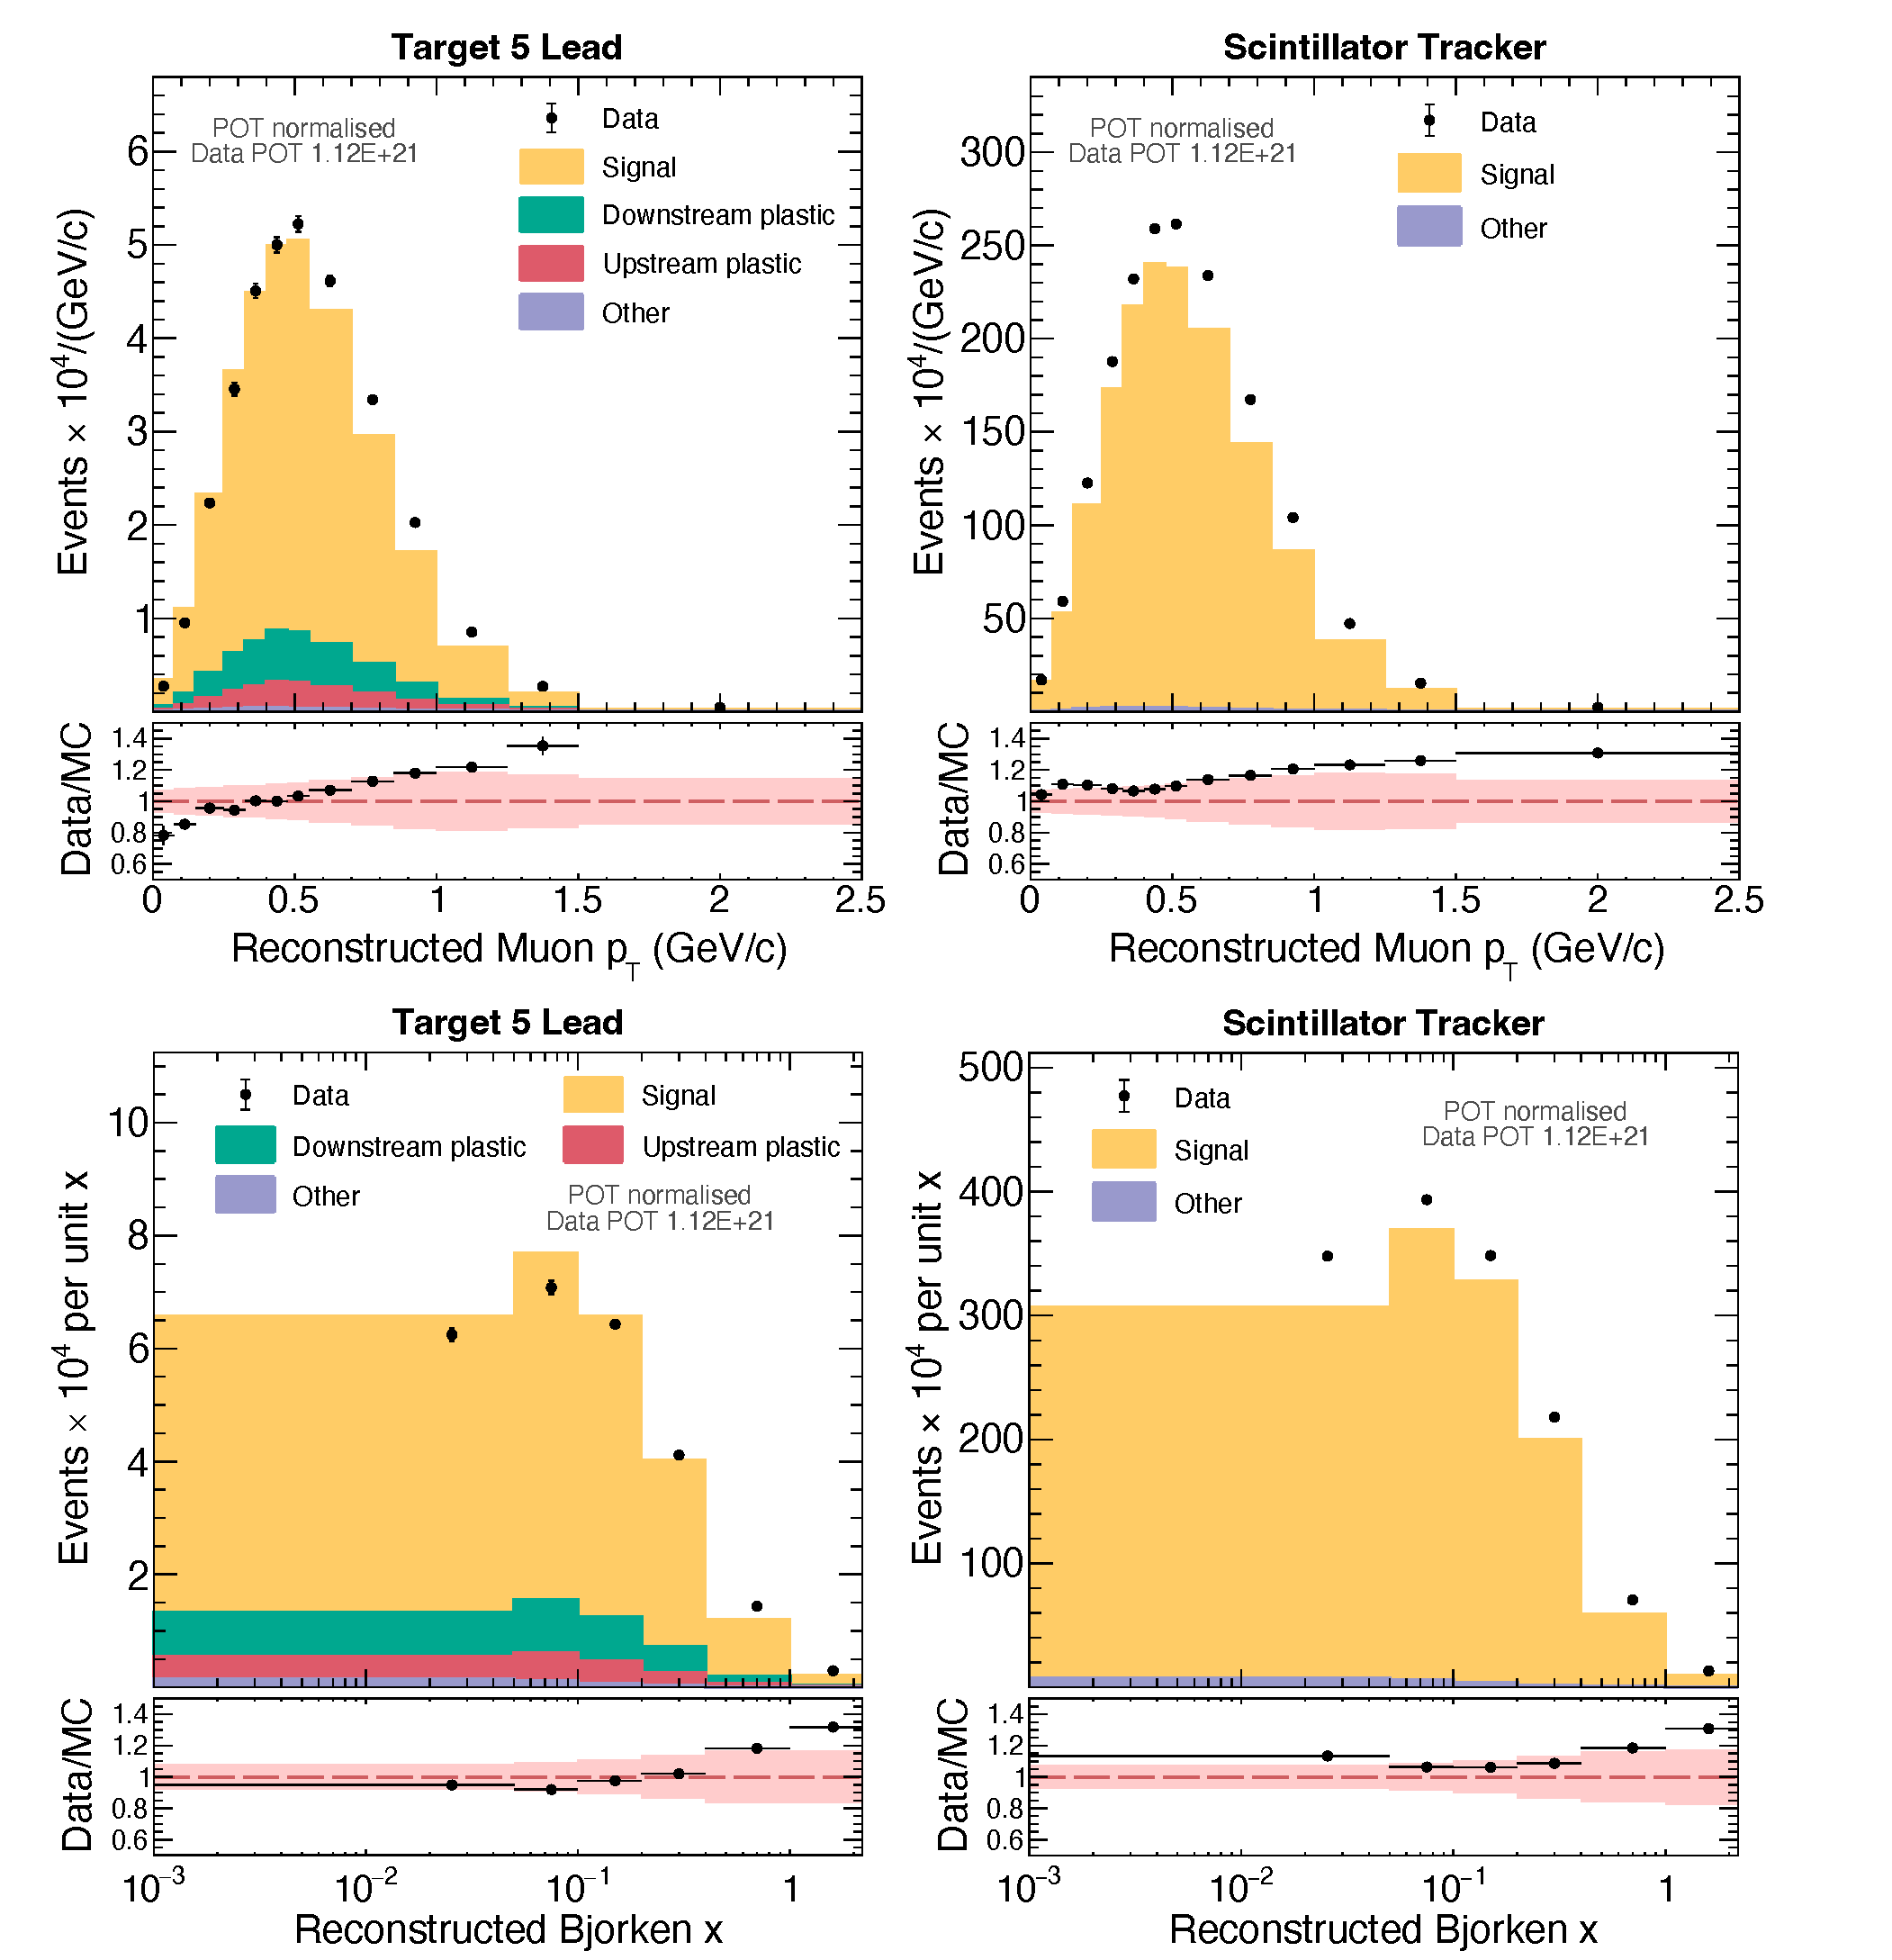
\includegraphics[width=1.\textwidth]{07analysis1D/figures/eventSelection_bkg_ratio_t5z82_tracker_pTx.pdf}}%
    \caption{Selected event distributions in target 5 lead (left panel) and the scintillator tracker (right panel) for both antimuon $p_{\text{T}}$ (top) and Bjorken $x$ (bottom). The distributions are bin-width and POT normalised. In the top panel of each plot, the black points represent the data with its statistical uncertainty, while the simulation is broken down into various sources of signal and background stacked in the descending order of their contribution. The bottom panel shows the data-to-simulation ratio. The solid band around the dashed line at 1 represents the systematic uncertainty on the simulation, while the black points carry the statistical uncertainty of the ratio. The horizontal lines on individual points indicate the bin width.}
    \label{fig:eventSelection_bkg_ratio_t5z82_tracker_pTx}
\end{figure}

Figure~\ref{fig:eventSelection_bkg_ratio_t5z82_tracker_pTx} illustrates a simulated breakdown of background in the reconstructed distribution for target 5 lead and the scintillator tracker, in both $p_{\text{T}}$ and Bjorken $x$. As depicted, the lower purity in targets, compared to the scintillator tracker, is a result of interactions reconstructed within the target that, in reality, occurred in the surrounding scintillator planes upstream (`Upstream plastic') and downstream (`Downstream plastic') of the relevant target. The `Other' category for targets combines events from different materials---for instance, in target 5 lead, it could include events from target 5 iron---and neutrino events contaminating the reconstructed charged-current antineutrino events. In the scintillator tracker, it combines the neutrino events with those from outside the tracker region instead. In both cases, it constitutes approximately 1\% of the reconstructed sample. The reconstruction cuts effectively eliminate any neutral current events. 

%Table~\ref{table:selectedEvents} also shows that the purity of nuclear target 4 and 5 is slightly lower than for the other targets. This is because they are thinner than the other nuclear targets as described in Chapter~\ref{ch:minerva}. Consequently, more events from the surrounding scintillator planes are prone to be misreconstructed in these thinner targets. 

It is also crucial to emphasize that there are no background events originating from outside the $x$--$y$ fiducial volume, the antimuon angle or the antimuon energy range depicted in Figure~\ref{fig:eventSelection_bkg_ratio_t5z82_tracker_pTx}. However, these backgrounds are appropriately accounted for in the final cross-section results through efficiency correction, allowing for their migration in and out of the sample during the unfolding procedure explained in Section~\ref{sec:migration_unfolding}. In practice, this involves applying the reconstruction cuts on the fiducial volume, energy, and angle range without utilizing the true information of the simulation for these aspects in the background subtraction, migration matrix, and efficiency numerator. The true information requirement is only included in the efficiency denominator.

Furthermore, the data-to-simulation ratio in Figure~\ref{fig:eventSelection_bkg_ratio_t5z82_tracker_pTx} serves as an initial indicator of how well the simulation predicts the data. While the simulation is tuned to encompass the latest measurements of neutrino pion production at MINERvA as described in Chapter~\ref{ch:dataAsimulation}, both the $p_{\text{T}}$ and Bjorken $x$ for target 5 lead and the scintillator tracker data distributions show a disagreement with the prediction, albeit in different ways.~All other selected event distributions with the background breakdown and the data-to-simulation ratios for the remaining nuclear targets of different materials are included in Appendix~\ref{ch:appendix_eventSelection}. 

The data distributions for the carbon-heavy scintillator tracker in both ${p_{\text{T}}}$ and Bjor\-ken~$x$ are generally higher than predicted by the simulation.~Nevertheless, the data mostly falls within the systematic uncertainties of the simulation prediction, except for the high ${p_{\text{T}}}$ and Bjorken $x$ region. The individual sources contributing to the systematic uncertainty band are discussed in Chapter~\ref{ch:systematics}. Similarly, the data distributions for target~3 carbon are also higher than the simulation prediction. The heavier iron targets show some agreement with the prediction at low ${p_{\text{T}}}$ and Bjorken $x$, but they are still underpredicted by the simulation at mid-to-high values of ${p_{\text{T}}}$ and Bjorken $x$. The data for the heavy lead targets exhibits a significant overprediction at low ${p_{\text{T}}}$ and Bjorken $x$, while still underpredicting the high ${p_{\text{T}}}$ and Bjorken $x$ region. In summary, the selected event distributions already indicate a significant nuclear dependence in antineutrino scattering which is not modelled by the simulation, especially in the low ${p_{\text{T}}}$ and Bjorken $x$ regions.

\begin{figure}[t!] 
    \centering
    {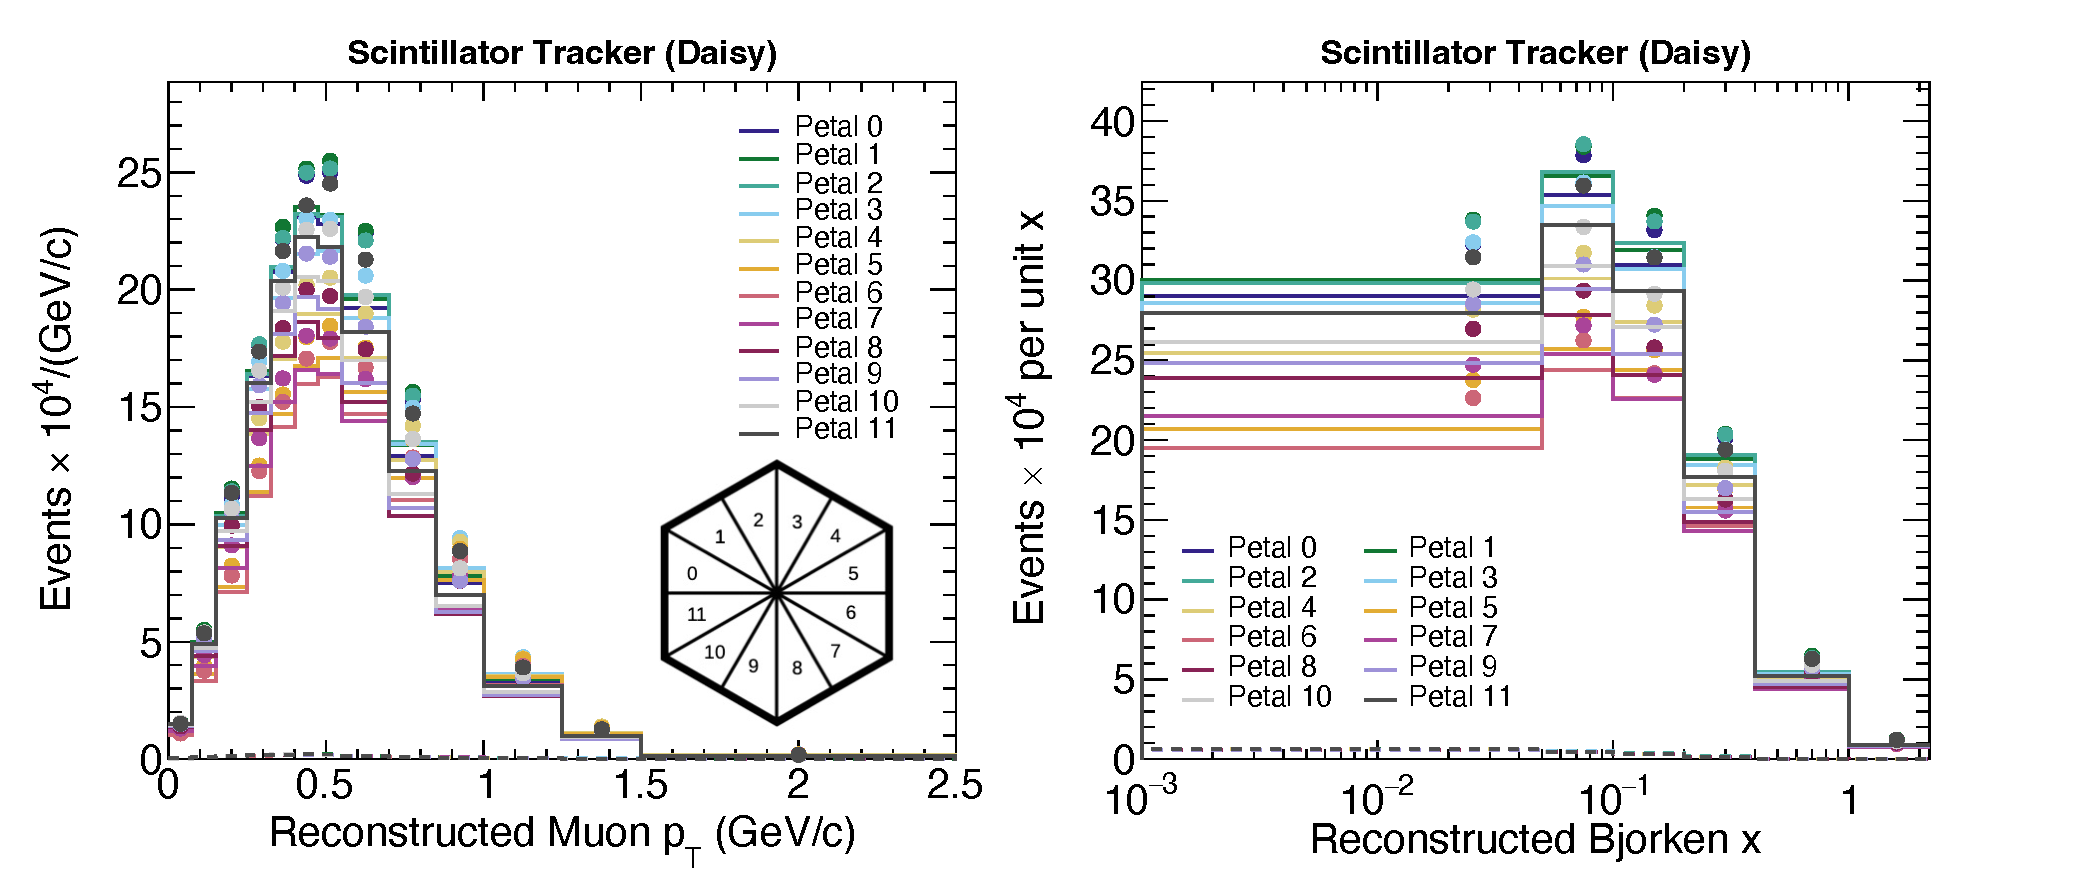
\includegraphics[width=1.\textwidth]{07analysis1D/figures/eventSelection_daisy_pTx.pdf}}%
    \caption{Selected event distribution for the scintillator tracker in `daisy petals' both in antimuon ${p_{\text{T}}}$ (left) and Bjorken $x$ (right). The simulation prediction for individual petals is depicted using coloured solid lines described in the legend, while the dashed lines show the simulated background prediction. For clarity, the uncertainty on the simulation is not shown. The corresponding points represent the data with its statistical uncertainty.~The hexagon insert illustrates petal positions looking downstream of the detector. }
    \label{fig:eventSelection_daisy_pTx}
\end{figure}

Finally, it is important to note that the scintillator tracker event distribution is also selected in 12 geometrical bins, referred to as ‘daisy petals’, as illustrated in Figure~\ref{fig:eventSelection_daisy_pTx} for both ${p_{\text{T}}}$ and Bjorken $x$. This extraction is essential for determining nuclear target-to-scintillator cross-section ratios using the matching flux technique discussed in Section~\ref{sec:nuclear_target_flux}. The number of events selected in each ‘daisy petal’ reflects the direction of the antineutrino beam traversing the detector. Additionally, ‘daisy petals' 5–7 experience a relative reduction in the number of events due to the MINOS coil cut.

\iffalse
Efficiency denominator - includes true angle cut and fiducial volume cut (x,y + separation). Angle and fiducial volume events are allowed to migrate in and out of the sample - efficiency corrected.
\fi
\newpage
\section{Background subtraction} \label{sec:bkgSubtraction}
% Here is a little trick because I am currently troubled with an issue 
% the cross-section for carbon when combine plastic sidebands and then 
% subtract vs use each plastic sideband separately and then combined background 
% subtracted stuff looks different
% Hence use: sidebands from the combined sidebands
% Background subtracted stuff from the seprate distributions so it's consistent... (somewhat lmao)
% Bkgs stuff from: /minerva/data/users/anezkak/10-25-2023_v430_p4/1D/combined/BackgroundSubtracted
% Sideband plots from: /minerva/data/users/anezkak/11-28-2023_v430_p4_combinedPlastic/1D/combined/PlasticSidebands


\newpage
\section{Migration and unfolding}
\label{sec:migration_unfolding}

\begin{figure}[b!] 
    \centering
    {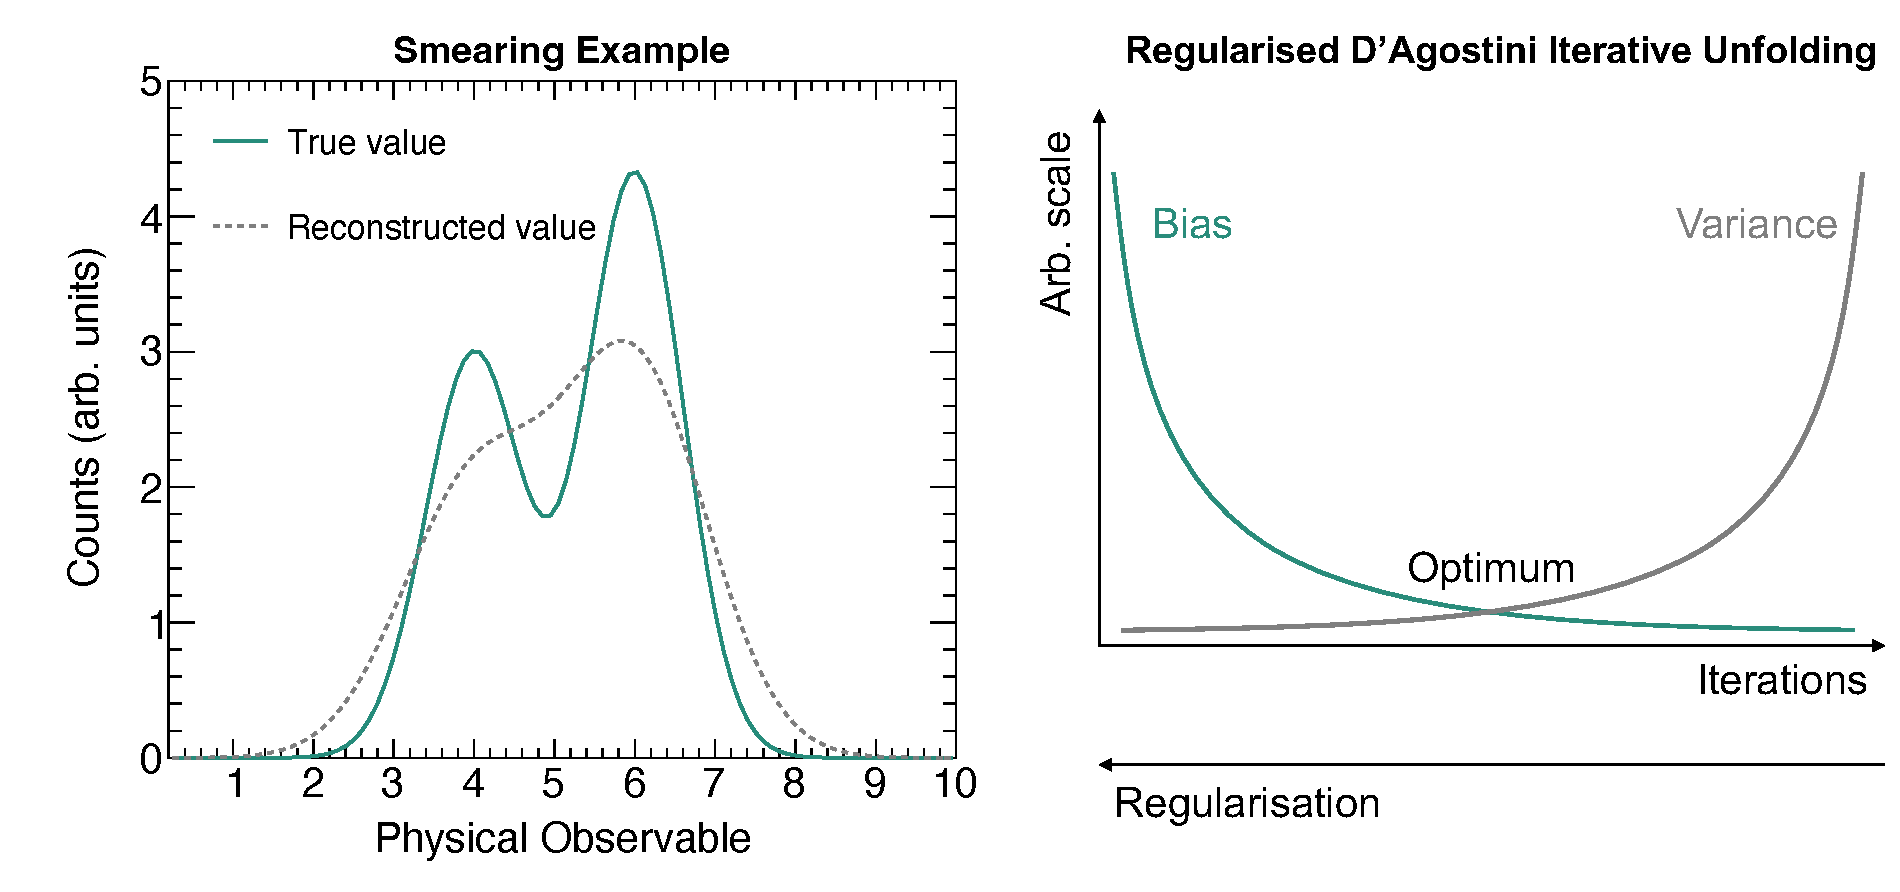
\includegraphics[width=1.\textwidth]{07analysis1D/figures/unfoldingExplanation_demo.pdf}}%
    \caption{Left: Smearing example of a two-component Gaussian model. The true histogram (solid line) shows more prominent peaks than the reconstructed histogram (dashed line) Right: Demonstration of the bias-variance trade-off in regularised D'Agostini iterative unfolding. Increasing the number of iterations leads to a less regularised solution with more variance. In practice, more variance also means that the statistical and systematic uncertainties increase rapidly. }
    % Intensities of the Poisson processes for the Gaussian mixture model data. Figure (a) shows the intensity function f of the true Poisson process and Figure (b) the intensity function h of the smeared Poisson process obtained by convolving the true intensity with a Gaussian of standard deviation σn = 1.2
    %[short caption] {long caption}
    \label{fig:unfolding_demo}
\end{figure}

Background-subtracted distributions offer the most accurate estimates of signal rates in reconstructed quantities. However, finite detector resolution and imperfect reconstruction may lead to deviations in the reconstructed kinematics of an event from its true kinematics, as demonstrated in Figure~\ref{fig:unfolding_demo}.~Put simply, there can be a difference between the actual physics that occurred and the physics that was measured. This effect, referred to as smearing, results in some events being reconstructed---or, in other words, migrated---into an adjacent or more distant bin than where they belong, smearing out the fine structure. The extent of this migration depends on how much lower or higher the reconstructed value is compared to the true value. The simulation sample, which contains both the true generated and the reconstructed information about the simulated events, is used to estimate the amount of smearing in data via a so-called migration matrix. 

%The migration matrix \textbf{$\text{K}^{\text{MC}}$} can be represented as a two-dimensional histogram relating the vector of bins of the true distribution $\boldsymbol{\lambda}$ on the $y$-axis and the vector of bins of the reconstructed distribution $\textbf{\text{n}}$ on the $x$-axis such as 
%\vspace{-10pt}
%\begin{equation}
%    \label{eq:smearing}
%    \vspace{-10pt}
%    n_{j} = \Sigma_{\alpha} K_{\alpha j}^\text{MC} %\lambda_{\alpha},
%\end{equation}
%using the known mapping.
The migration matrix can be represented as a two-dimensional histogram relating bin~$\alpha$ of the true generated distribution on the $y$-axis to bin $j$ of the reconstructed distribution on the $x$-axis, $U_{j\alpha}$. The more diagonal the matrix is, the less smeared the reconstructed distribution is. Examples of migration matrices for target~5 lead and the scintillator tracker in both $p_{\text{T}}$ and Bjorken $x$ are shown in the Figure~\ref{fig:migration_lead_tracker_pTx}. It is important to note that the migration matrices also consider underflow and overflow bins, which include values below or above the lowest and highest bin boundaries. This accounts for smearing in and out of the sample; however, these bins are not explicitly shown in Figure~\ref{fig:migration_lead_tracker_pTx}. All other migration matrices for passive targets and the scintillator tracker divided in the geometrical bins, i.e. `daisy petals', are included in Appendix~\ref{ch:appendix_migrationMatrices}.

\begin{figure}[b!] 
    \centering
    {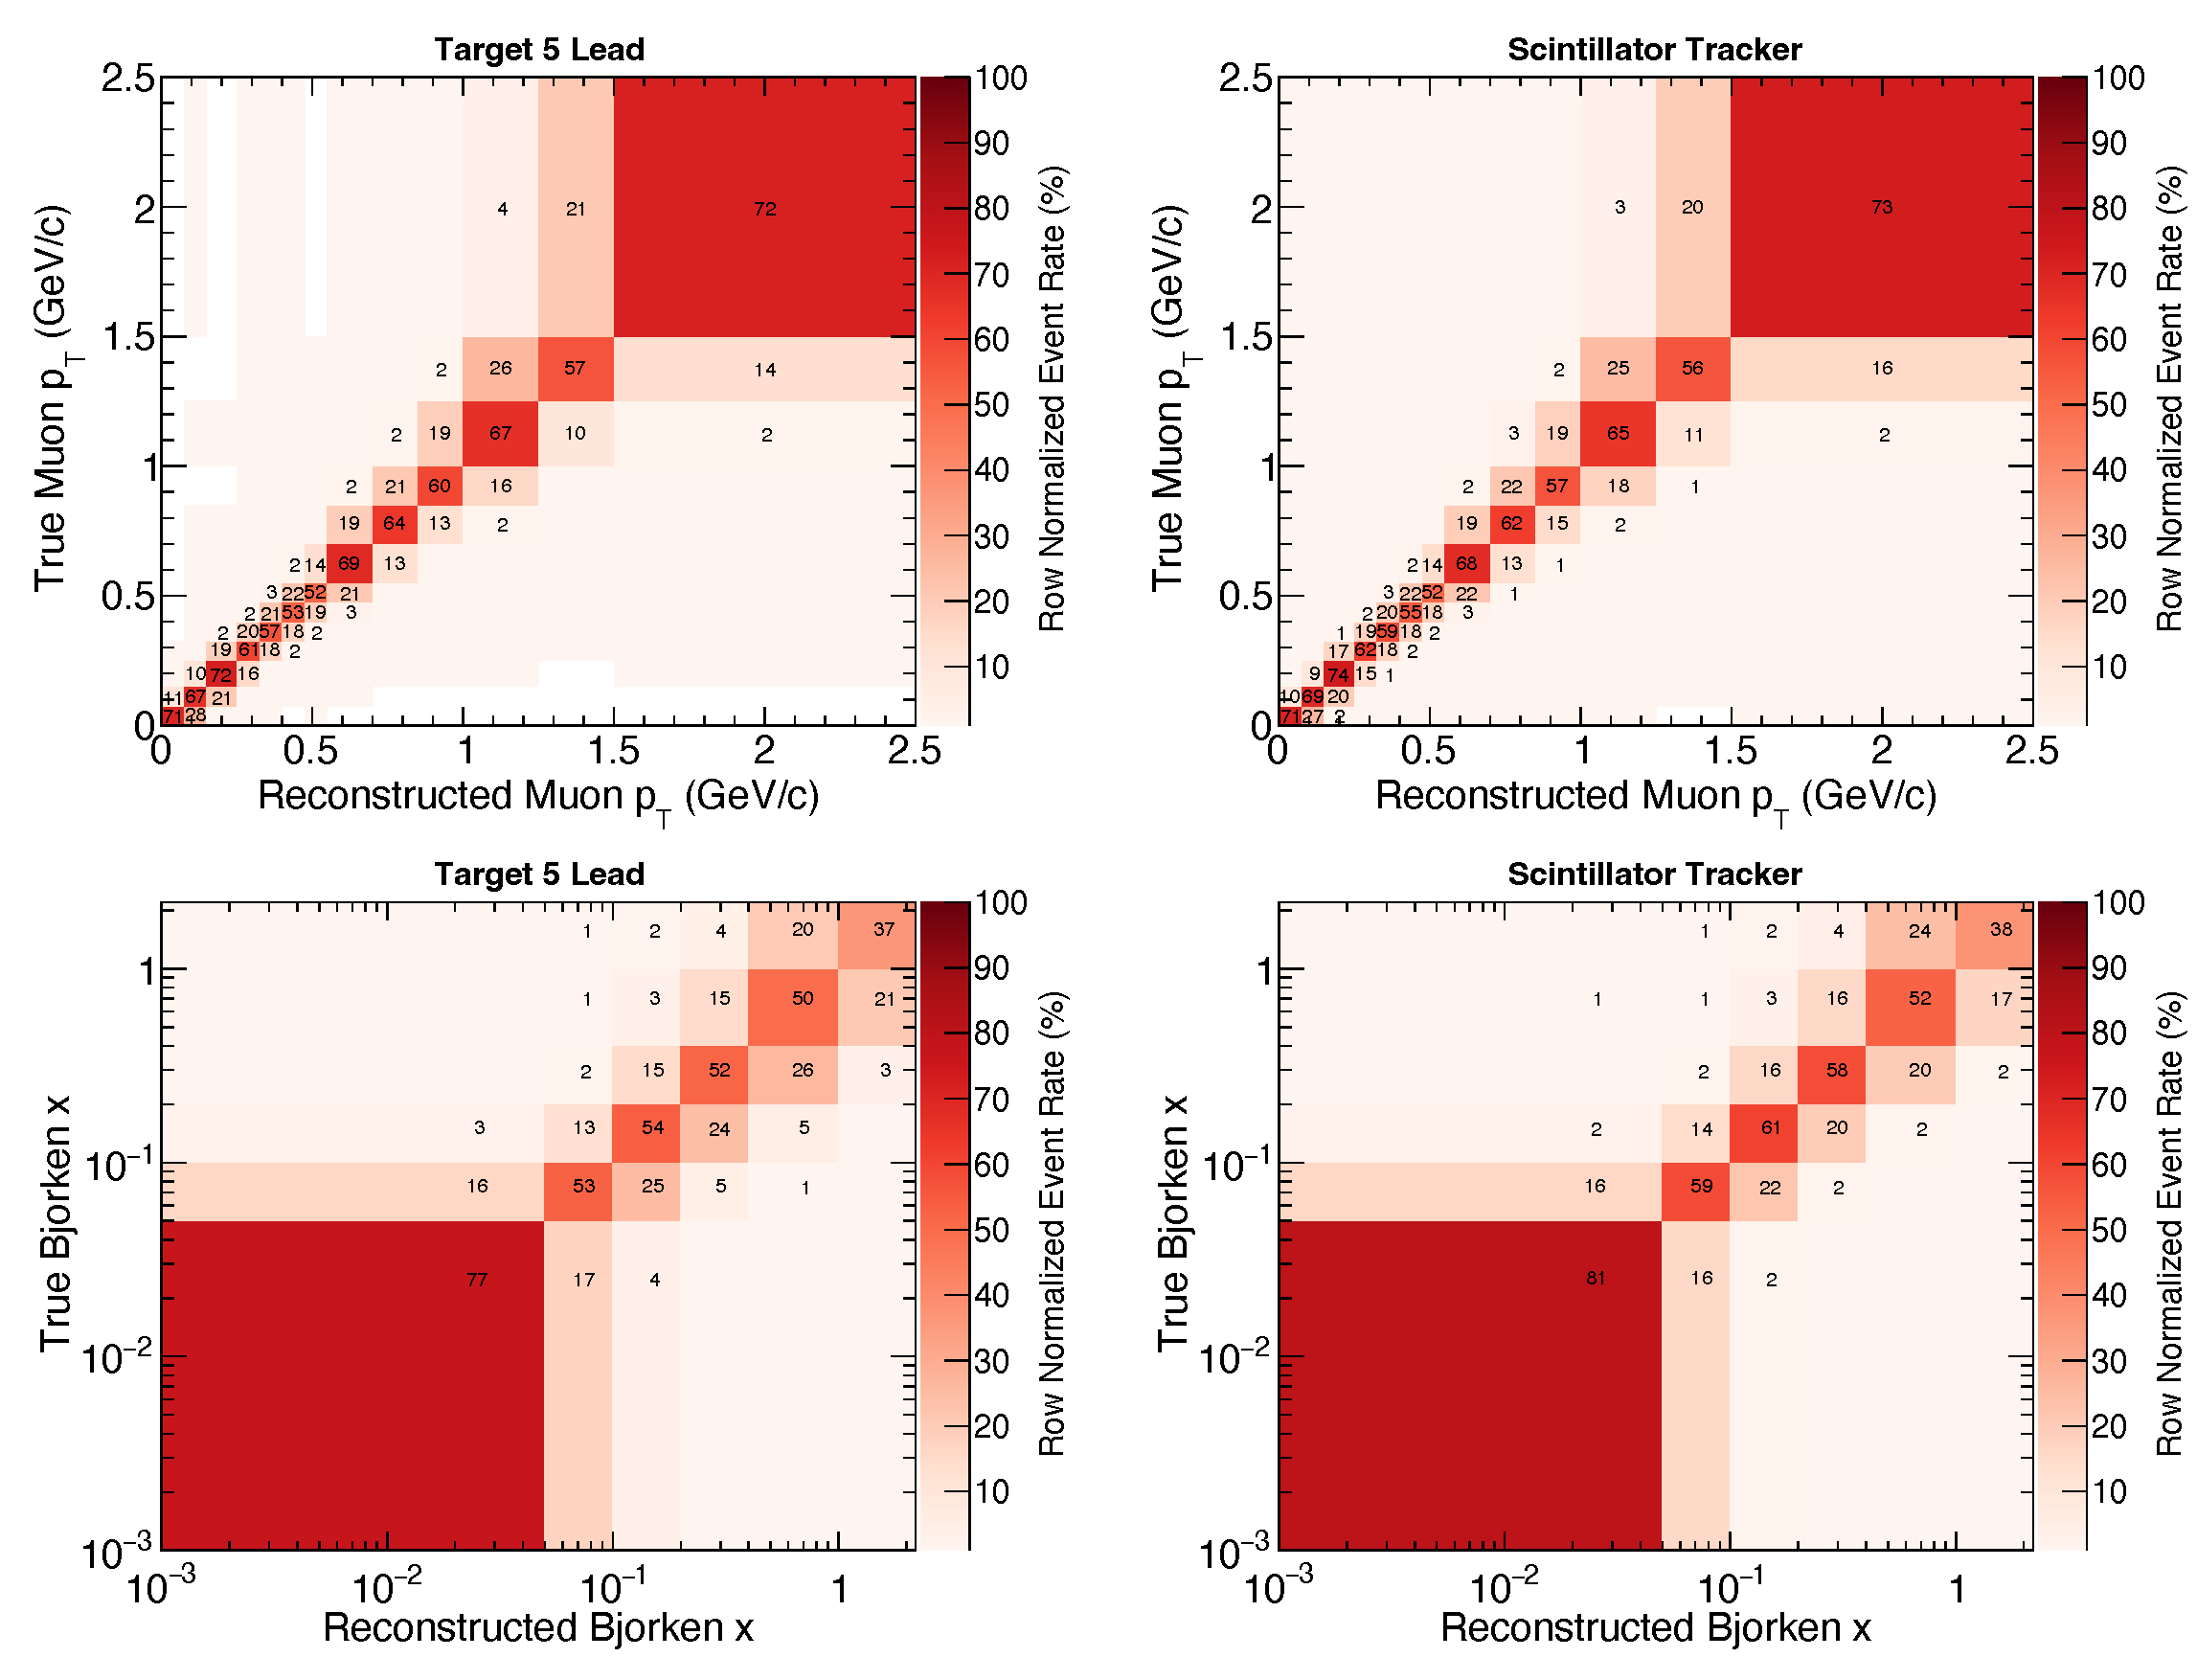
\includegraphics[width=1\textwidth]{07analysis1D/figures/migration_lead_tracker_pTx.pdf}}%
    \caption{Row-normalised migration matrices for target 5 lead (left panel) and scintillator tracker (right panel) both in $p_{\text{T}}$ (top) and Bjorken $x$ (bottom). Each row of the migration matrix is normalised to 1 to represent the probability that an event generated in a given bin $\alpha$ will be reconstructed in a bin $j$.}
    %[short caption] {long caption}
    \label{fig:migration_lead_tracker_pTx}
\end{figure}

The $p_{\text{T}}$ distribution is primarily smeared by the finite muon momentum resolution of the detector, stemming from the size of the scintillator strips affecting the length of particle tracks. On the other hand, the Bjorken $x$ distribution smearing likely arises from the calorimetric correction used to estimate the invisible energy from neutrons in the hadronic recoil energy reconstruction, as described in Chapter~\ref{ch:Reconstruction}. In addition, the region with $x > 1$, discussed in Chapter~\ref{ch:measurement}, is already inherently challenging at the true simulation level.~Events in this region predominantly originate from intranuclear scattering, and may not necessarily include other physics contributions such as short-range correlations indicated by electron-scattering data~\cite{CLAS:PhysRevLett.96.082501,SRC:annurev}. Therefore, caution is exercised when working with this particular bin. In general, the migration matrices are more diagonal in the scintillator tracker than in the passive target region due to better tracking (more active material). 


%and relying on the simulation to estimate the smearing effects in the data.
% needs a reference for electron-scattering
% My x > 1 region studies:
% https://minerva-docdb.fnal.gov/cgi-bin/sso/RetrieveFile?docid=29951&filename=collabMeeting_December2021.pdf&version=1
% https://minerva-docdb.fnal.gov/cgi-bin/sso/RetrieveFile?docid=29808&filename=October-2021_update_inclusives.pdf&version=1
% annual review

In order to report a detector-independent cross-section, the smearing of the reconstructed distribution must be reversed. The process of estimating the true distribution from the measured smeared spectrum is called unfolding. Unfolding the distributions is crucial for future reinterpretations of the result, combinations with other experiments, and aiding the understanding of various physics models. In the cross-section extraction Equation~\ref{eq:xsec1D}, the unfolding process is denoted by $\Sigma_{j} \tilde{U}_{j\alpha}$ acting on bin $j$ of the background subtracted reconstructed distribution.

% UNFOLDING IS AN ILL POSED PROBLEM
% Cowan, G. Statistical Data Analysis (Oxford University Press Distribution Services North Kettering Business Park Hipwell Road Kettering Northants NN14 1UA, 1998).
% https://indico.cern.ch/event/107747/contributions/32645/attachments/24317/35000/blobel.pdf
\begin{comment}
\begin{figure}[b!] 
    \centering
    {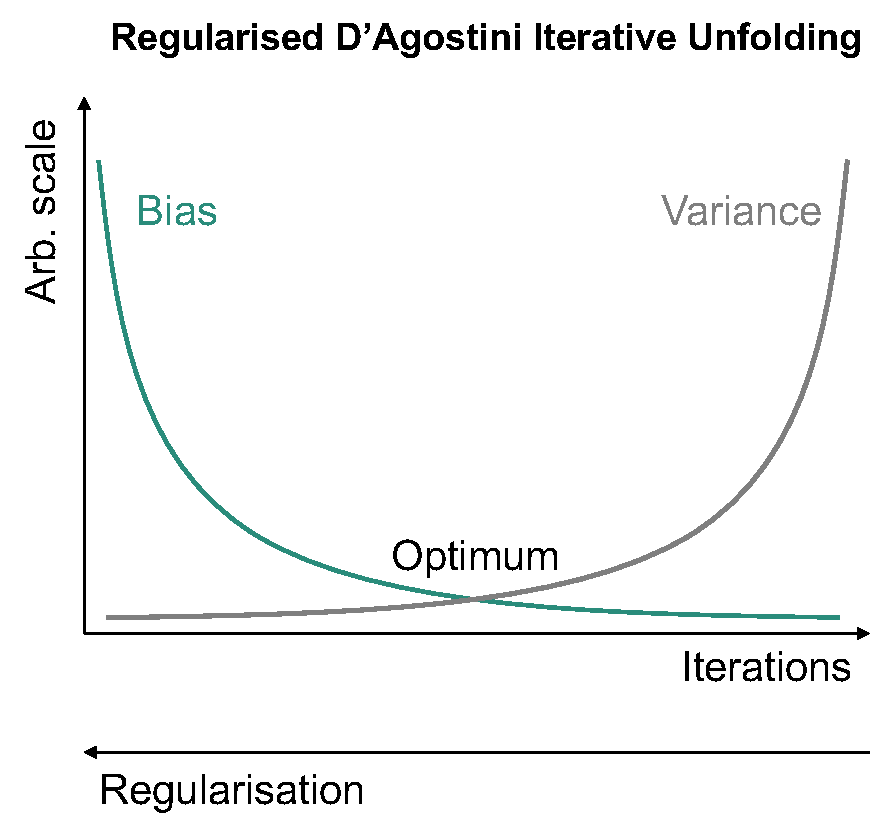
\includegraphics[width=0.8\textwidth]{07analysis1D/figures/unfoldingExplanation.pdf}}%
    \caption{Demonstration of the bias-variance trade-off in regularised D'Agostini iterative unfolding. Increasing the number of iterations leads to a less regularised solution with more variance. In practice, more variance also means that the statistical and systematic uncertainties increase rapidly. }
    %[short caption] {long caption}
    \label{fig:unfolding_explanation}
\end{figure}
\end{comment}

Unfolding could be achieved by inverting the migration matrix, which is, however, not always invertible. Moreover, unfolding is, by definition, an ill-posed problem as small changes in the measured distribution can lead to significant fluctuations in the true distribution, i.e.~large variance \cite{blobel2002unfolding}. Introducing regularisation in the unfolding process can address this issue by trading off some variance for a controlled amount of bias\footnote{Bias is defined as the difference between the expected value of the unfolded result and the true unmeasured expected value, which in the simulation is the true generated value.}. Similar to other MINERvA results, this analysis uses the D'Agostini iterative regularisation method~\cite{DAgostini:1994fjx,DAgostini:2010hil} implemented in the RooUnfold package~\cite{Adye:2011gm} in ROOT~\cite{ROOT_Brun:1997pa}, where the regularisation parameter is the number of iterations, as illustrated in Figure~\ref{fig:unfolding_demo}.
% Kevin McFarland:
%https://minerva-docdb.fnal.gov/cgi-bin/sso/RetrieveFile?docid=15224&filename=Unfolding%20MINERvA.pdf&version=2
% Kuusela unfolding
% https://infoscience.epfl.ch/record/220015?ln=en

%Uy=lambda
% lambda is truth
% y is measured data
% U is the migration matrix
% simulation-truth dependent. unfolding matrix is iteratively improved and applied to the data to give and improved estimate
The $(k+1)$th iteration of the D'Agostini method is determined by 
\vspace{-10pt}
\begin{equation}
    \label{eq:unfolding}
    \vspace{10pt}
    \lambda_{\alpha}^{(k+1)} = \frac{\lambda_{\alpha}^{(k)}}{\sum_{j=1}^N U_{j\alpha}} \mathlarger{\sum}_{j=1}^N \frac{U_{j\alpha}y_j}{\sum_{\beta=1}^P U_{j\beta}\lambda_{\beta}^{(k)}},
\end{equation}
where $U_{j\alpha}$ is the simulation-based migration matrix, $\lambda_{\alpha}^{(k)}$ represents the vector of bins of the true distribution at iteration $k$, and $y_{j}$ is the vector of bins of the reconstructed distribution.~In RooUnfold, the initial prior $\boldsymbol{\lambda}^{(0)}$ is the simulation prediction of the true distribution, i.e. $\boldsymbol{\lambda}^{(0)}$ = $\boldsymbol{\lambda}^{\text{MC}}$~\cite{Adye:2011gm}.~A more detailed description of the method can be found in the Appendix~\ref{ch:appendix_unfolding}.

In practice, the unfolding procedure is independently applied to both the central value histogram and all systematic universes. Since any statistical variation in the reconstructed distribution can be interpreted as a smearing of the fine structure of the true distribution, unfolding the distribution using many iterations results in the statistical and systematic uncertainties increasing rapidly. Therefore, it is crucial to determine the optimal number of iterations demonstrated in Figure~\ref{fig:unfolding_demo}, balancing the aforementioned reduction of bias while keeping variance minimal.~MINERvA analyses find this number of iterations via so-called warping studies.

Unfolding the underlying simulation with the migration matrix based on that simulation would result in perfect unfolding in one iteration, leading to maximum modelling bias. Therefore, warping studies involve the unfolding of fake data, referred to as `warped models'. These warped models are simulations that have been reweighted to depict alternative physics models, exaggerate features of the underlying distributions, or capture differences in the shapes of distributions between the data and the original underlying simulation. The reconstructed distributions of warped models, where the truth is known, are unfolded using a migration matrix based on the original underlying simulation. The number of iterations is then determined by looking at the least number of iterations required for $\chi^2$, defined as 
%\vspace{-10pt}
\begin{equation}
    \label{eq:unfolding}
    %\vspace{-10pt}
    \chi^2= \sum_{\alpha, \beta} \left( \lambda^{(k)}-\lambda \right)_{\beta}V^{-1}_{\beta\alpha}\left( \lambda^{(k)}-\lambda \right)_{\alpha},
\end{equation}
to stabilise near minimum, i.e.~the number of degrees of freedom of the distribution. Here, $ \lambda^{(k)}$ is the unfolded distribution after $k$ iterations in bin $\alpha$ or $\beta$, $\lambda$ is the true value of the distribution and $V$ is the unfolding covariance matrix.

\begin{table}[b!]
    \centering

    \begin{tabular}{c p{10cm}}
    \hline\\ [-1.5 ex]
    Warped Model & Description \\ [0.5ex] % inserts table %heading
    \hline\hline\\[-1.7ex]
    Resonant $M_{A}^{\text{RES}}$ nominal & Resonant axial mass $M_{A}^{\text{RES}}$ and CCResNorm in the Rein-Seghal model described in \ref{subsec:pionProduction} are set to their GENIE nominal values, i.e. $M_{A}^{\text{RES}}$ = $1.12$~GeV/$c^2$  and CCResNorm = 1.0 \\ % 3.78413e+29 \\
    \hline
    Non-resonant pion production & Non-resonant pion production reduction described in Section~\ref{subsec:pionProduction} is varied within its $1\sigma$, i.e.~reduction to 47\% of its nominal value (rather than to 43\%) \\
    \hline
    Valencia 2p2h enhancement off & Nominal Valencia 2p2h model, i.e.~the 50\% enhancement over the nominal prediction of Valencia 2p2h described in Section~\ref{subsec:2p2h} is not used \\ %9.59755e+28 \\
    \hline
    SuSA 2p2h & Valencia 2p2h is reweighted to the Super-Scaling Approximation (SuSA) 2p2h model~\cite{PhysRevD.94.093004} according to Refs.~\cite{PhysRevD.101.033003,SuSAreweight_MINERvA} (without the 2p2h enhancement)\\%4.27675e+29 \\
    \hline
    Bjorken $x$ ratio & Central value is reweighted according to a fitted smooth function to the background subtracted data/MC ratio in the tracker, i.e.~1st-degree polynomial as a function of true Bjorken~$x$ with a constant value equal to the ratio value of the centre of the last bin above the centre of the last bin (1.6).
     \\ %3.23478e+30 \\
    \hline
    Antineutrino energy ratio & Same as above except using a fitted 3rd-degree polynomial as a function of true antineutrino energy, constant and equal to the ratio value of the centre of the last bin above the centre of the last bin (19~GeV). \\ %3.23478e+30 \\
    \hline
    \end{tabular}

    \caption{List of warped models used to determine to number of iterations of the D'Agostini unfolding.}
    \label{table:warpingList}
\end{table}

Warping studies are performed purely as statistical studies, meaning only the central values of reconstructed distributions are considered. To address statistical fluctuations, central values of warped models are used to generate 100 Poisson-distributed statistical universes with a mean of the number of warped model entries in each bin, and the distributions are unfolded in each of these statistical universes. The list of conducted warping studies can be found in Table~\ref{table:warpingList}.

Pion production is one of the largest contributions to this medium-energy antineutrino-inclusive sample. Therefore, two warped models affecting the pion production---`Resonant $M_{A}^{\text{RES}}$ nominal' and `Non-resonant pion production' listed in Table~\ref{table:warpingList}---were chosen to investigate the potential unfolding instabilities and to assess the model dependence on the underlying simulation. Furthermore, two different models for the 2p2h sample were tested, specifically the base Valencia 2p2h (`Valencia 2p2h enhancement off') and the alternative 2p2h model based on the Super-Scaling Approximation (`SuSA 2p2h')~\cite{PhysRevD.94.093004}. The choice of these models was motivated particularly by the impact of neutrons in final states from the 2p2h interaction on the high Bjorken $x$ distribution.~Finally, the two last warped models listed in the Table~\ref{table:warpingList} are data/MC ratio warps. These warps were implemented to examine potential unfolding issues arising from differences between the underlying simulation and the data, a critical consideration given that data unfolding relies on the simulation.
% My warping studies
% March 2023
% https://minerva-docdb.fnal.gov/cgi-bin/sso/RetrieveFile?docid=31540&filename=11-03-2023-collabMeeting.pdf&version=1
% June 2023
% https://minerva-docdb.fnal.gov/cgi-bin/sso/RetrieveFile?docid=31766&filename=presentation.pdf&version=1
% August
% https://minerva-docdb.fnal.gov/cgi-bin/sso/RetrieveFile?docid=31913&filename=2023-08-04-unfolding_x_v430.pdf&version=2
%https://minerva-docdb.fnal.gov/cgi-bin/sso/RetrieveFile?docid=31954&filename=2023-08-24-update.pdf&version=1 


The warping studies in Table~\ref{table:warpingList} were conducted for each kinematic distribution in every target. The same warping studies were also replicated for each of the geometrical bins, referred to as `daisy petals', of the scintillator tracker distribution used in the nuclear target to scintillator cross-section ratios using the matching flux technique discussed in Section~\ref{sec:nuclear_target_flux}.~Generally, the warping studies showed that the passive target region requires one more iteration to unfold than the scintillator tracker. However, to maintain consistency across various materials for each kinematic distribution, the number of iterations was standardized across all warping studies. All antimuon $p_{\text{T}}$ distributions were unfolded with 3 iterations of the D'Agostini unfolding, and all Bjorken $x$ distributions were unfolded with 9 iterations as listed in the Table~\ref{table:unfoldingIterations}.

\begin{table}[b!]
    \centering

    \begin{tabular}{c c}
    \hline \\ [-1.5 ex]
    Variable & Number of iterations \\ [0.5ex] % inserts table %heading
    \hline\hline
    $p_{\text{T}}$ & 3 \\ %9.59755e+28 \\
    %\hline
    Bjorken $x$ & 9 \\ % 3.78413e+29 \\
    \hline
    \end{tabular}

    \caption{Number of iterations used in the D'Agostini unfolding of antimuon $p_{\text{T}}$ and Bjorken~$x$ determined by the warping studies to extract final cross-sections.}
    \label{table:unfoldingIterations}
\end{table}

\begin{figure}[b!] 
    \centering
    {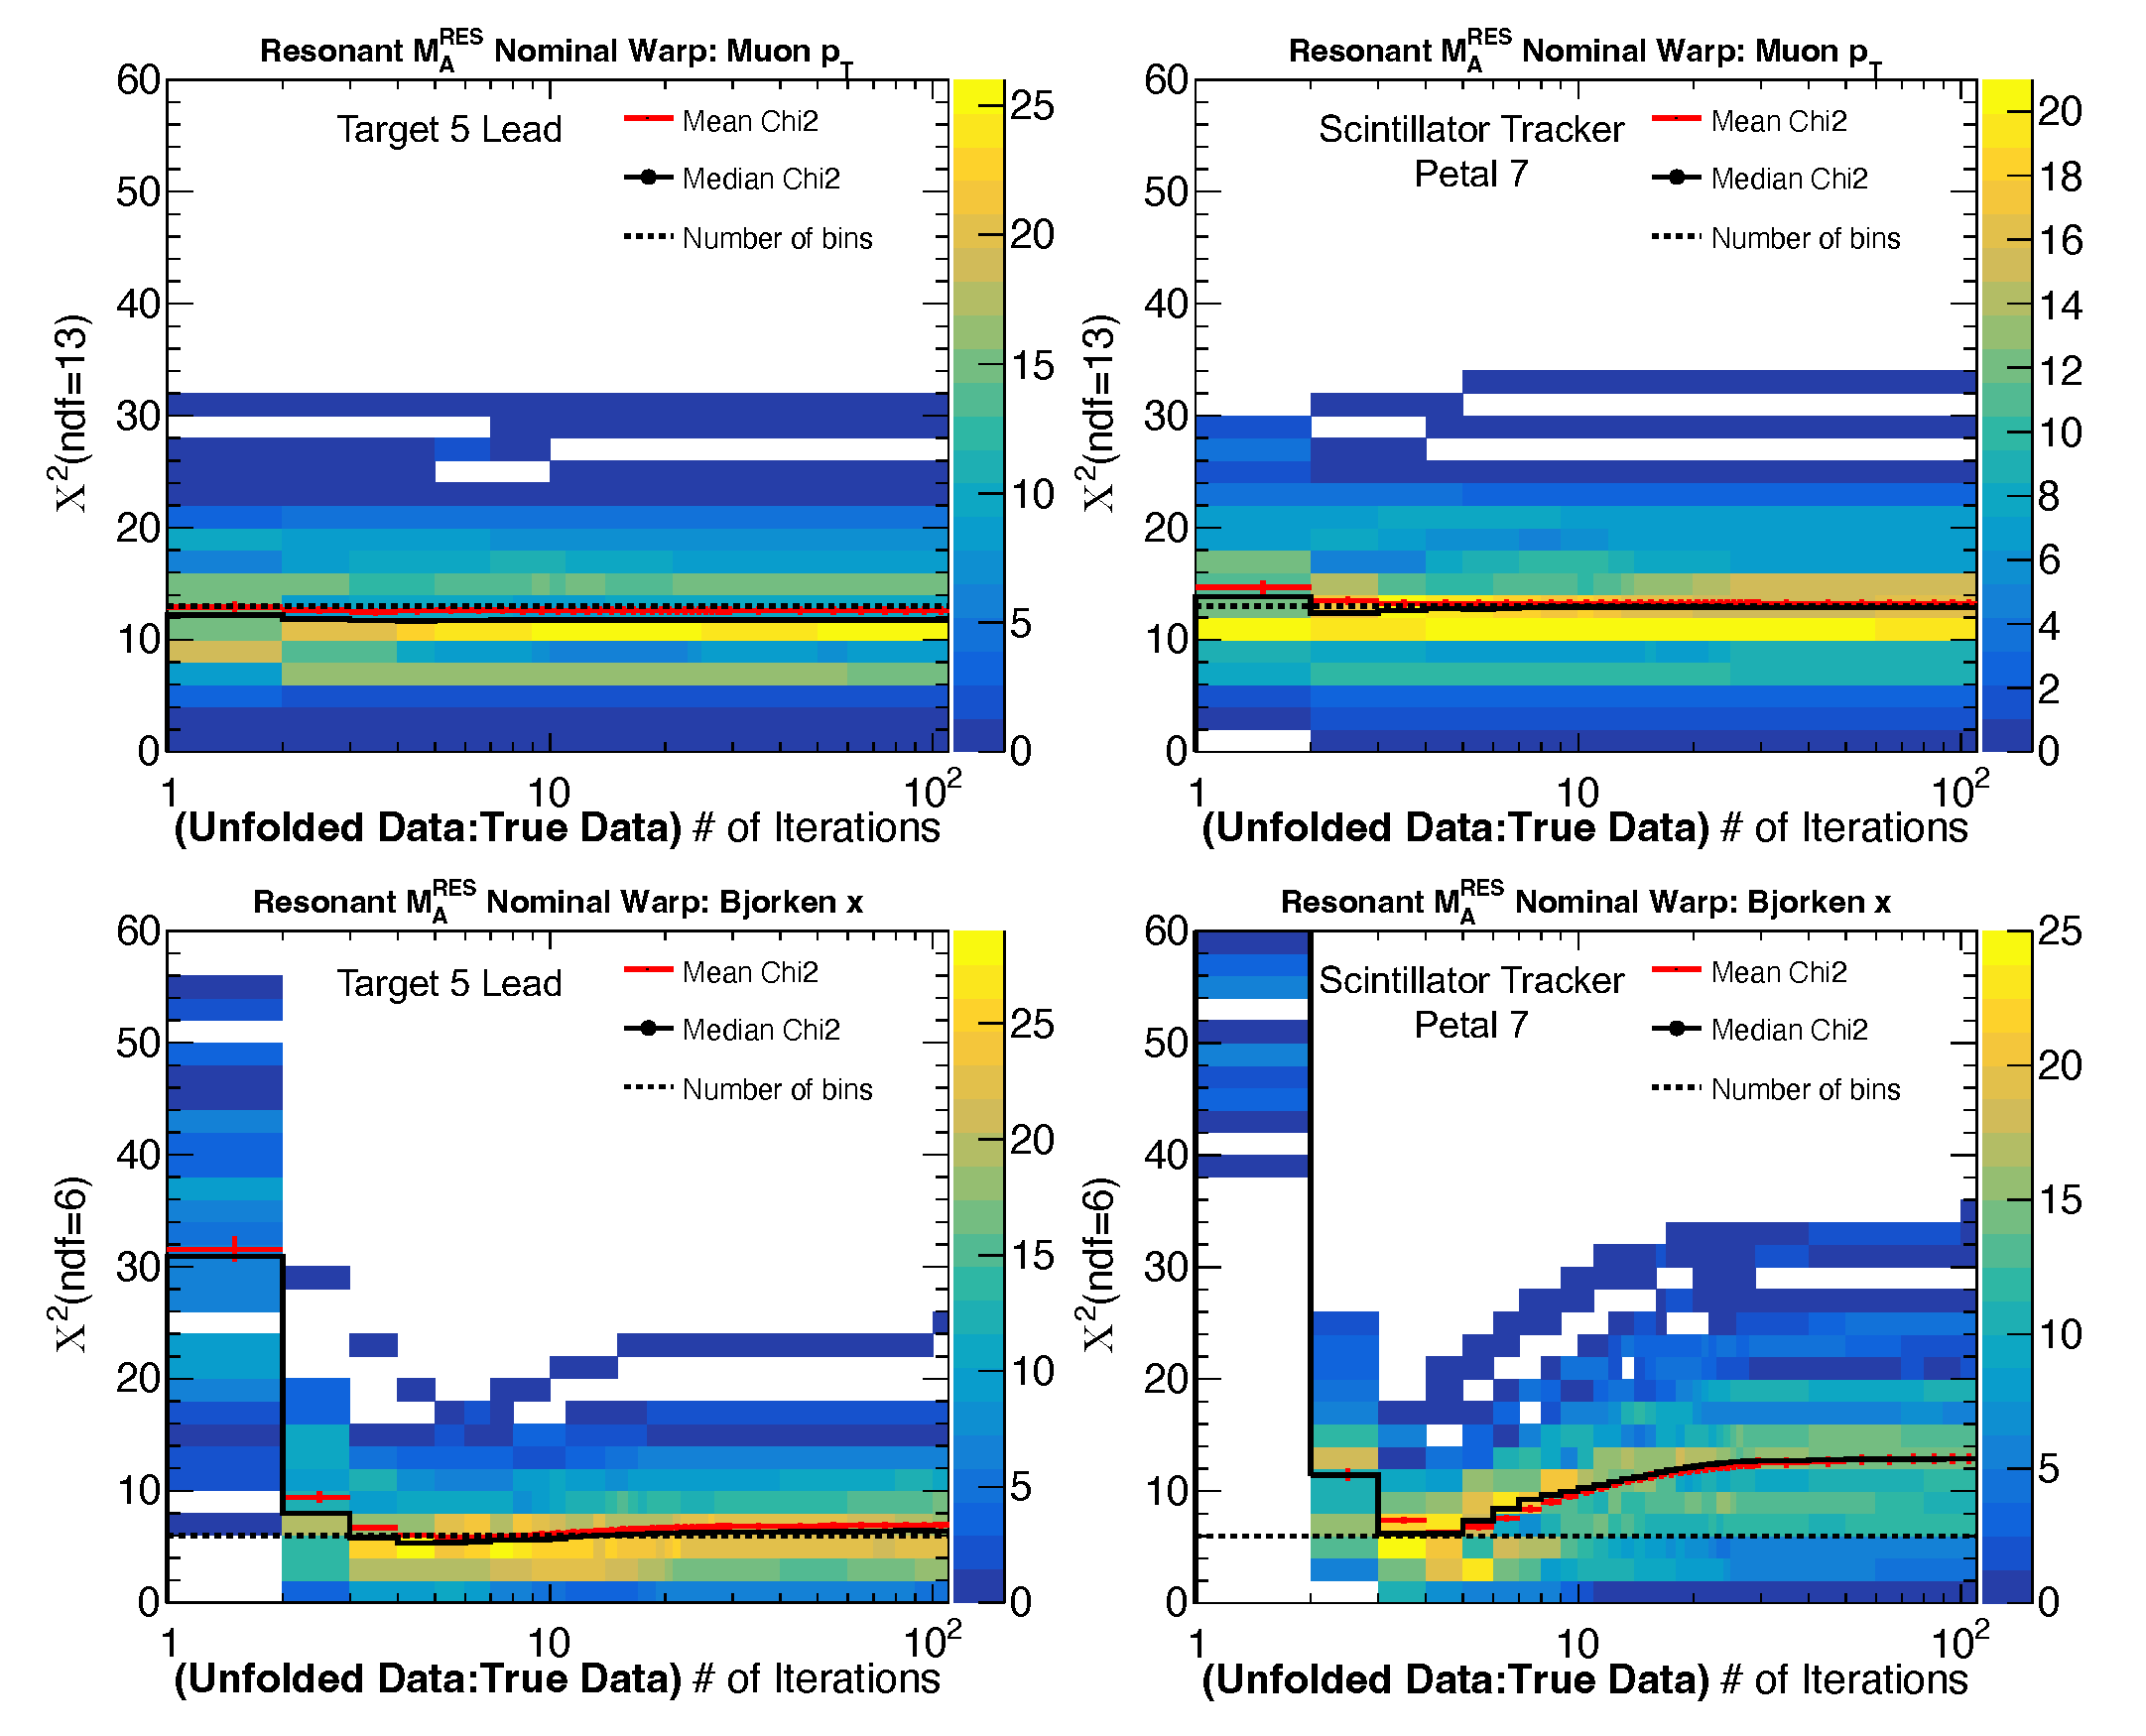
\includegraphics[width=1\textwidth]{07analysis1D/figures/maresWarp_lead5tracker7_pTx.pdf}}%
    \caption{The 'Resonant $M_{A}^{\text{RES}}$ nominal' warping study conducted for target 5 lead (left panel) and the scintillator tracker petal 7 (right panel) in both antimuon $p_{\text{T}}$ (top) and Bjorken $x$ (bottom). Each heatmap displays the calculated $\chi^2$ between the unfolded and true distribution of the warped model as a function of the number of iterations for each of the 100 Poisson throws. The solid lines represent the median and mean $\chi^2$, while the dashed line indicates the number of bins or degrees of freedom (ndf). In $p_{\text{T}}$, the median $\chi^2$ quickly approaches the ndf, signalling minimal bias. In contrast, the median $\chi^2$ for Bjorken $x$ converges to the ndf more gradually. The bottom right heatmap for the scintillator tracker petal 7 exhibits a 'check-mark' shape, indicating convergence to a minimum and then a slight divergence. This pattern prompted further investigation into potential model dependence.}
    %[short caption] {long caption}
    \label{fig:warpingMaRes}
\end{figure}

An example of the `Resonant $M_{A}^{\text{RES}}$ nominal' warping study for target 5 lead and the scintillator tracker petal 7 both in antimuon $p_{\text{T}}$ and Bjorken $x$ is shown in Figure~\ref{fig:warpingMaRes}. While the median $\chi^2$ for $p_{\text{T}}$ is not very far off from the number of degrees of freedom to begin with and converges almost immediately, the Bjorken $x$ median $\chi^2$ has the typical shape of a warping study---each iteration brings the $\chi^2$ closer to the number of degrees of freedom. Furthermore, the scintillator tracker petal 7 distribution in Bjorken $x$ has a `check-mark' shape, where the median $\chi^2$ dips to a minimum at the number of degrees of freedom and then slightly diverges to about twice the number of degrees of freedom over several iterations. To investigate the potential model dependence (and given this is not a blind analysis), the data cross-section was extracted with the warped model as an alternative central value employing the standard cross-section extraction procedure described in this chapter with 9 iterations of unfolding for Bjorken $x$ as listed in the Table~\ref{table:unfoldingIterations}. The data cross-section unfolded with this alternative model was compared to the cross-section extracted with the original simulation to show that the central values of the alternative model are covered by the total (and also just the systematic---outer error bars) uncertainty, and hence any potential model dependence is accounted for by the overall uncertainty. For clarity, this is demonstrated in Figure~\ref{fig:maresCheck_invisECheck} as a lead-to-scintillator cross-section ratio with the individual cross-section comparisons and other cross-section ratio comparisons included in the Appendix~\ref{ch:appendix_unfoldingStudies}.

\begin{figure}[t!] 
    \centering
    {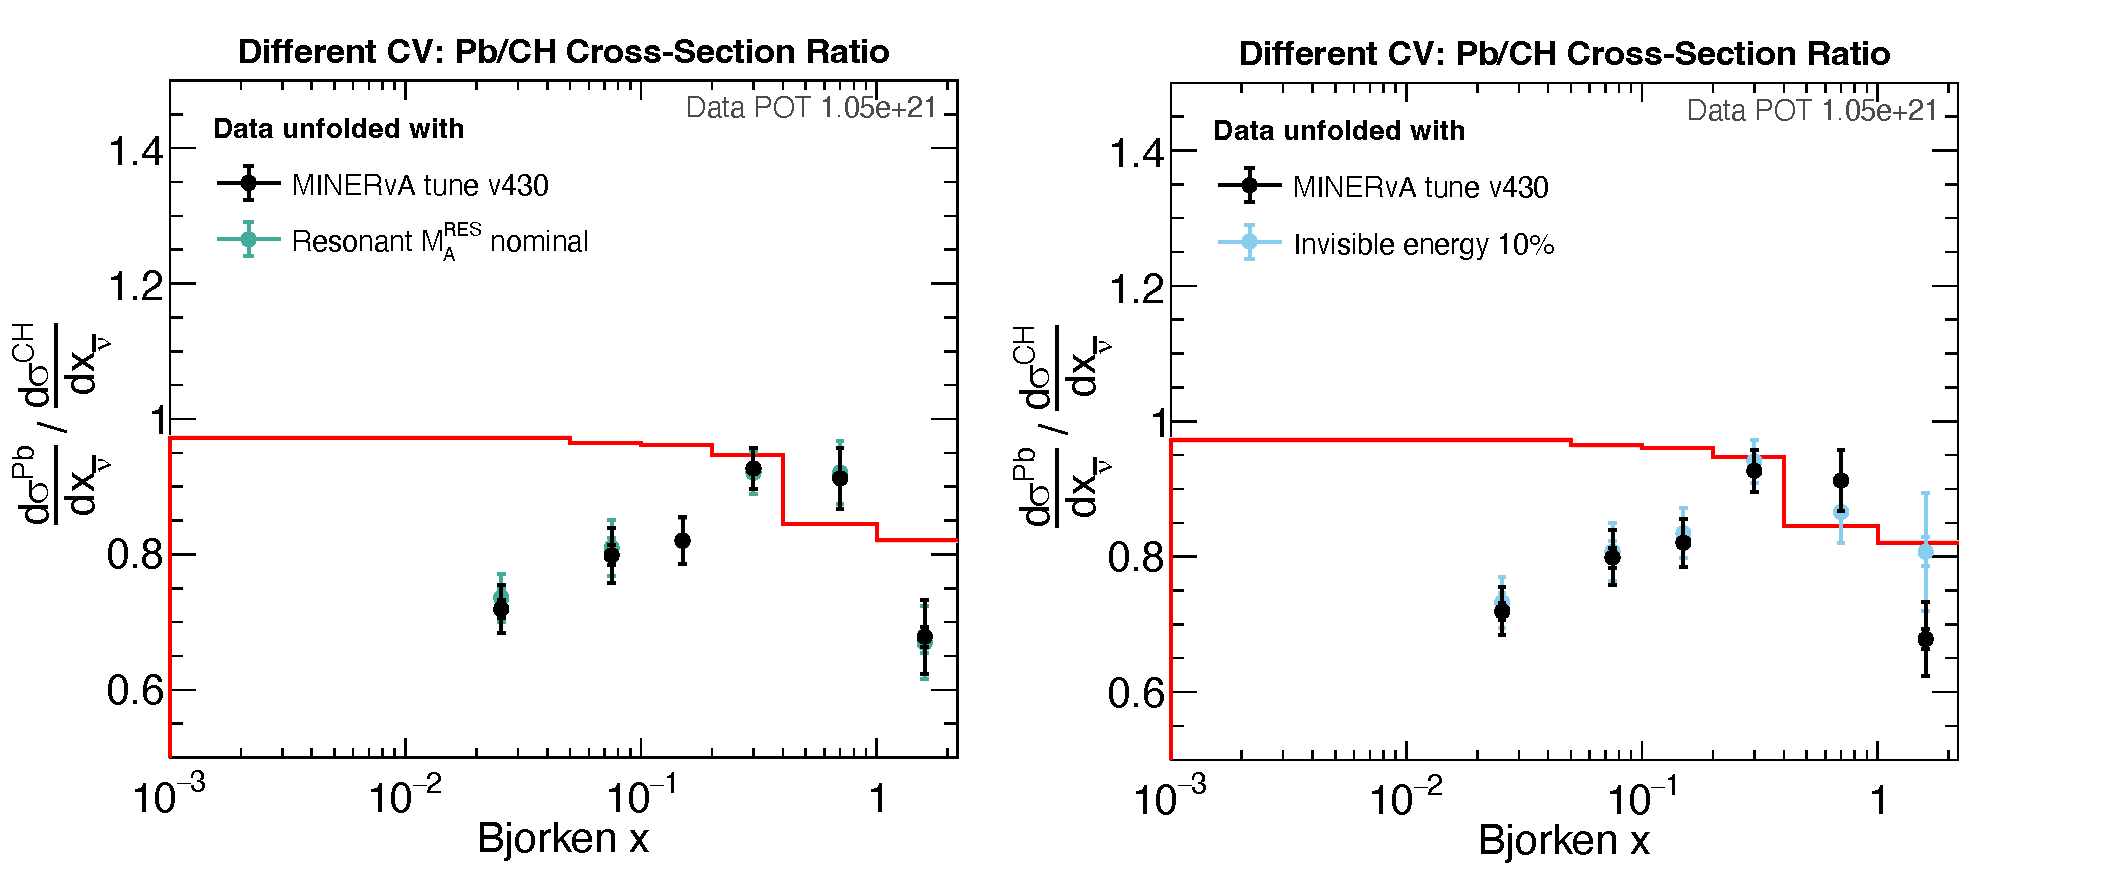
\includegraphics[width=1\textwidth]{07analysis1D/figures/maresCheck_invisECheck.pdf}}%
    \caption{Left: Comparison of the lead-to-scintillator data cross-section ratio extracted with the underlying simulation MINERvA tune v430 and the warped model `Resonant $M_{A}^{\text{RES}}$ nominal' as a function of Bjorken $x$. The central values of the data cross-section extracted using the warped model are encompassed by the total uncertainty (including the systematic, represented by the outer error bars) of the data cross-section extracted using the original simulation. This indicates that any potential model dependence is covered by the underlying uncertainty. Right: Comparison of the  lead-to-scintillator data cross-section ratio as a function of Bjorken $x$ extracted with the original simulation and `Invisible energy 10\%' central value to investigate model dependence arising from neutron modelling, revealing possible bias in the $x > 1$ bin.}
    %[short caption] {long caption}
    \label{fig:maresCheck_invisECheck}
\end{figure}

The `SuSA 2p2h' warping study for the same targets (target 5 lead and the scintillator tracker petal 7) in both $p_{\text{T}}$ and Bjorken $x$ is also shown in the Figure~\ref{fig:warpingSuSA_pulls} using the calculated mean of the pull distribution in each bin at various numbers of iterations. The pull of a kinematic distribution in each bin $i$ is defined as
\vspace{-10pt}
\begin{equation}
    \label{eq:pulls}
    \vspace{-10pt}
    \text{pull}_{i} = \frac{(\text{reco}-\text{true})_i}{\sigma_{i}^{\text{true}}},
\end{equation}
where `reco' is the reconstructed value, `true' is the unfolded value and $\sigma_{i}^{\text{true}}$ is the uncertainty on the unfolded value in the given bin $i$. This visualisation of the warping study also illustrates that the `SuSA 2p2h' warped model can be unfolded using the central value migration matrix for both $p_{\text{T}}$ and Bjorken $x$. The pull distributions nicely represent how with each iteration the unfolding gets less biased, i.e. the mean of the pull distribution in every bin gets closer to zero. The equivalent distribution to Figure~\ref{fig:warpingMaRes} for the `SuSA 2p2h' warped model and the pull distribution for the `Resonant $M_{A}^{\text{RES}}$ nominal' warp are included in the Appendix~\ref{ch:appendix_unfoldingStudies}.

\begin{figure}[b!] 
    \centering
    {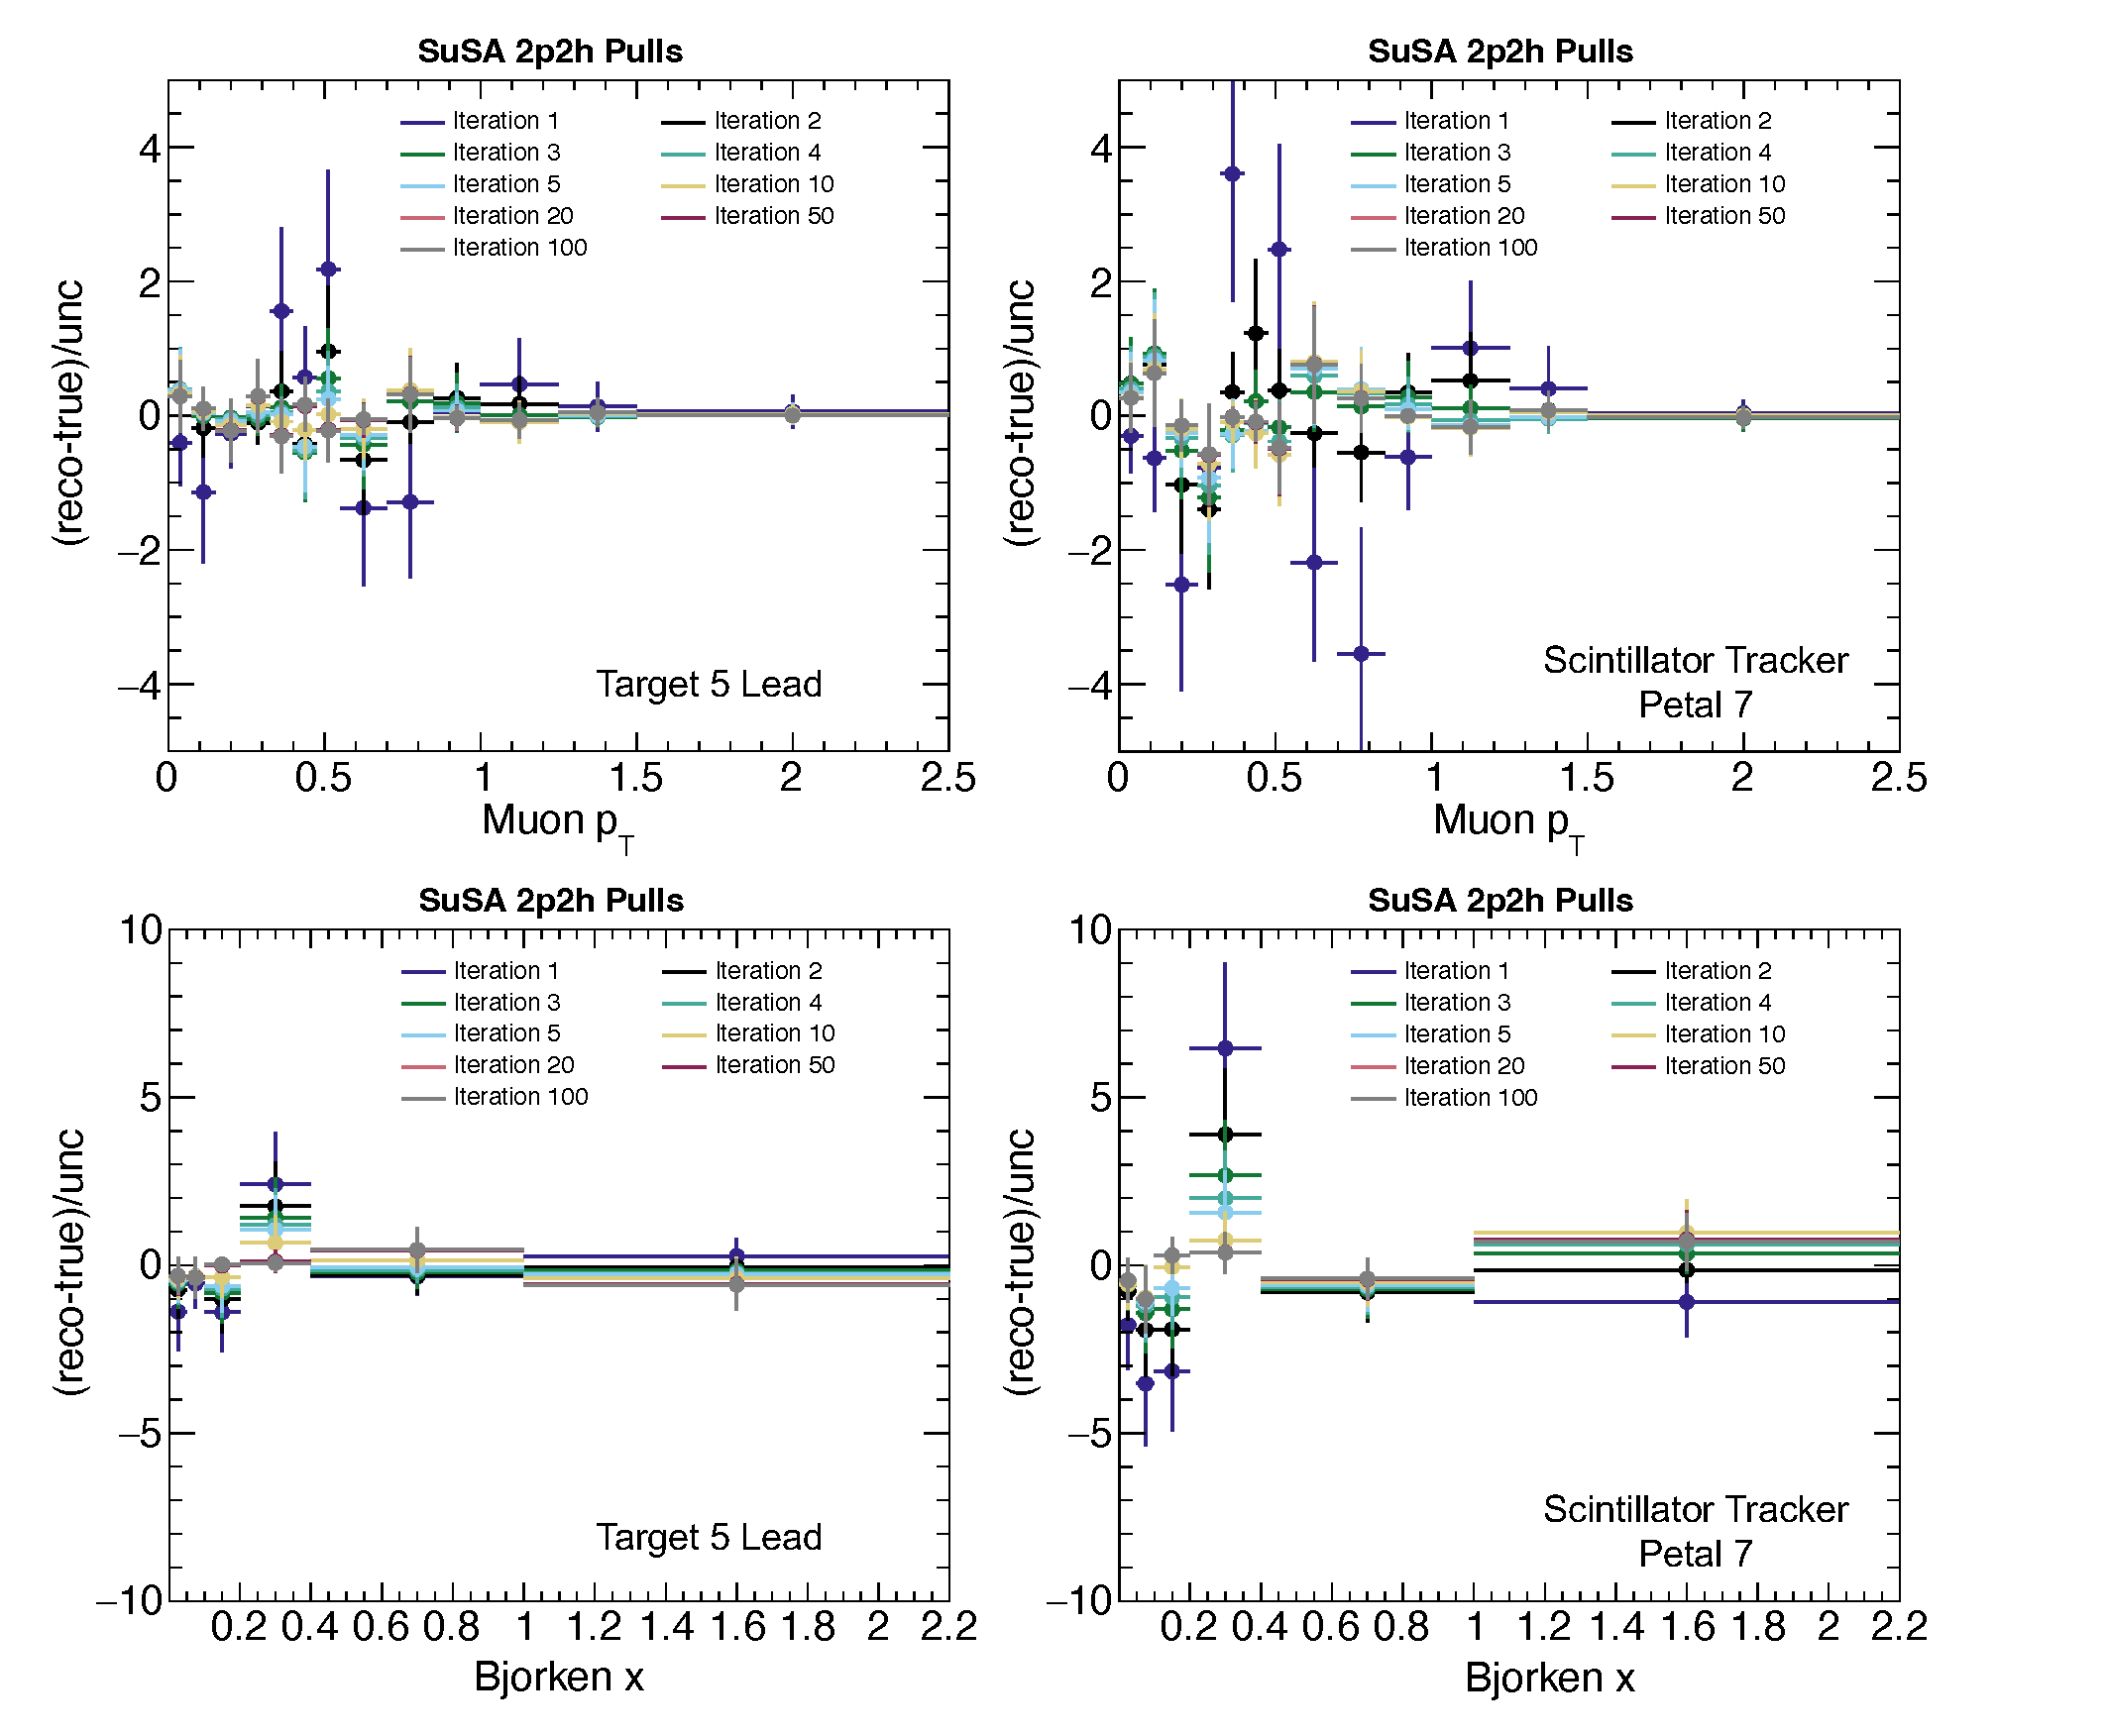
\includegraphics[width=1\textwidth]{07analysis1D/figures/susaWarp_lead5tracker7_pTx_pulls.pdf}}%
    \caption{Pull distributions for the 'SuSA 2p2h' warping study for target 5 lead (left panel) and the scintillator tracker petal 7 (right panel) in both antimuon $p_{\text{T}}$ (top) and Bjorken $x$ (bottom). Each pull distribution illustrates the reduction in bias with each iteration of the unfolding process.~In other words, the mean of the pull distribution in each bin converges toward zero.}
    %[short caption] {long caption}
    \label{fig:warpingSuSA_pulls}
\end{figure}

Apart from the warping studies detailed in Table~\ref{table:warpingList}, an additional simple study was conducted to evaluate the potential bias introduced by neutron production in antineutrino interactions in this analysis.~This is particularly relevant as antineutrino interaction generators are typically employed to correct for these effects, given that most of the energy deposited by neutrons in detectors is invisible. However, a recent MINERvA measurement of multi-neutron cross-sections showed disagreement with predictions from several leading models \cite{MINERvA:2023ikp}. Hence, the neutron modelling corrections introduced at the unfolding level could impact the Bjorken $x$ distribution, especially in the high $x$ region, where they are coupled with the already inherently challenging modelling of the $x > 1$ region mentioned earlier in this chapter.

Thus, the strategy was to examine how a change at the true level of the simulation (and not the reconstructed) impacts the analysis.~Naïvely, this was accommodated by introducing additional invisible energy into the system, achieved by increasing the true antineutrino energy by 10\% of the true invisible energy while keeping the muon system intact. Similar to the investigation of the bias in the case of the `check-mark' shaped warping study discussed above, the data cross-section was extracted with this new model using 9 iterations of unfolding for Bjorken $x$ and compared to the cross-section extracted using the original simulation. The lead-to-scintillator cross-section ratio in Figure~\ref{fig:maresCheck_invisECheck} shows that the central values of the alternative model are covered by the total uncertainty, except for the last $x > 1$ bin. This potential source of model bias requires further action, and the possibility of including an additional source of systematic uncertainty related to neutron modelling is discussed in Chapter~\ref{ch:systematics}. The individual cross-section comparisons and the other cross-section ratio comparisons can be found in Appendix~\ref{ch:appendix_unfoldingStudies}.

\begin{figure}[t!] 
    \centering
    {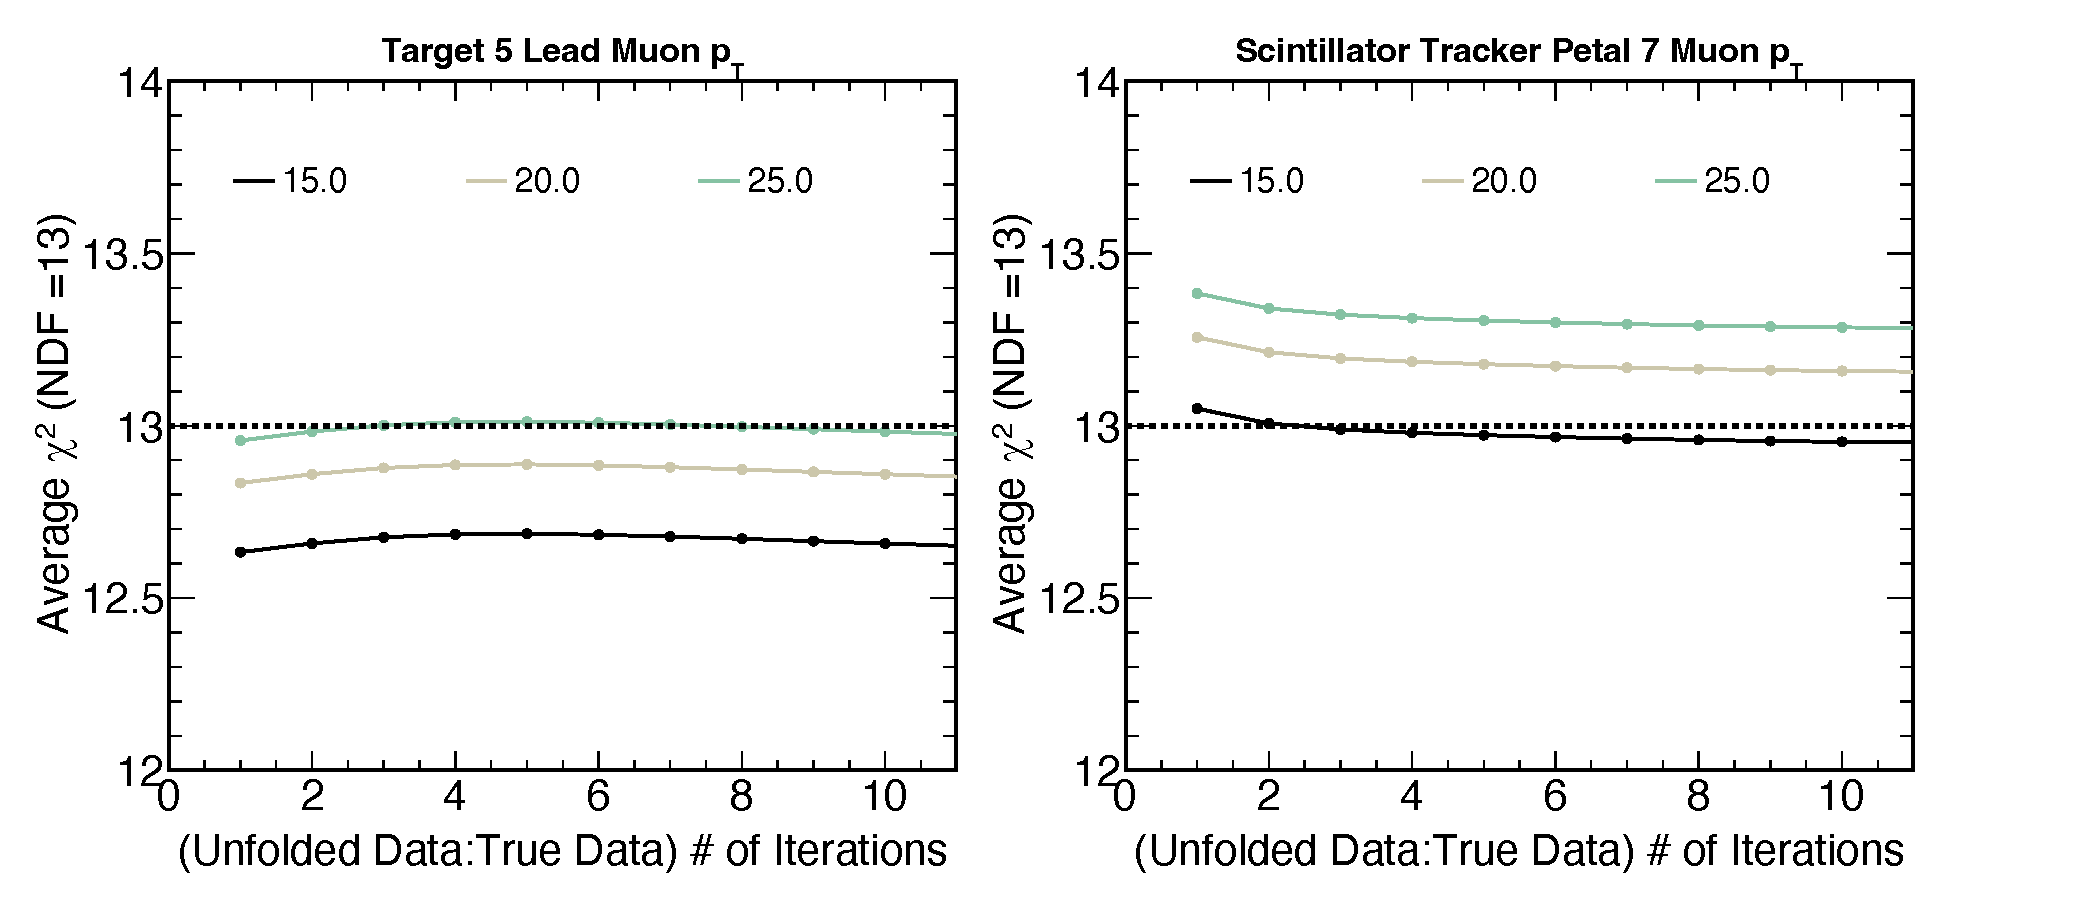
\includegraphics[width=1\textwidth]{07analysis1D/figures/additionalStatUnc_lead5tracker7_pT.pdf}}%
    \caption{Correction factor $F$ to the statistical uncertainty of the unfolded sample due to finite size of the simulation in the migration matrix for target 5 lead and the scintillator tracker petal 7 in antimuon $p_{\text{T}}$. The solid lines illustrate that at the selected number of iterations, i.e. 3 iterations, the calculated $\chi^2$ between the unfolded and true simulation converges to the number of degrees of freedom (dashed line) for the $F$ factor 25 and 15 for the target 5 lead and the scintillator tracker petal 7 respectively.  }
    %[short caption] {long caption}
    \label{fig:additionalStatUnc_pT}
\end{figure}

Finally, RooUnfold's implementation of the D'Agostini unfolding doesn't take into account uncertainties in the response matrix due to the finite statistics of the simulation sample~\cite{Adye:2011gm}. This leads to an underestimation of the statistical uncertainty of the unfolded sample and can be particularly significant for large sample analyses such as this one. To address this issue, a correction factor to the statistical uncertainty related to the relative simulation-to-data fraction, i.e.~about 4.43 for the antineutrino dataset used in this analysis, was implemented. 

% https://minerva-docdb.fnal.gov/cgi-bin/sso/RetrieveFile?docid=28899&filename=MINERvA_Unfolding_AMatterOfUncertainty.pdf&version=1
% https://minerva-docdb.fnal.gov/cgi-bin/sso/RetrieveFile?docid=28992&filename=MINERvA_Unfolding_AMatterOfUncertainty_FollowUp_Collaboration.pdf&version=2

In order to do so, a new migration matrix was constructed by Poisson throwing each bin of the original migration matrix as a fraction of data exposure. Then, the new reconstructed simulation coming from the projection of the new migration matrix was unfolded with this new migration matrix and compared to the original true \mbox{simulation~\cite{StatCorrFactor,StatCorrFactor2}}. The statistical covariance of the unfolded sample was multiplied by $\sqrt{(1+1/F)}$, where $F$ is the correction factor. 
A search over various $F$ factors for the given fraction of data exposure was performed such as the calculated $\chi^2$ between the unfolded sample with the corrected statistical covariance and the original true distribution corresponded to the number of degrees of freedom at the number of iterations selected. Figure~\ref{fig:additionalStatUnc_pT} illustrates the correction factors $F$ for the antimuon $p_{\text{T}}$ distributions in target 5 lead and the scintillator tracker petal 7, which are 25 and 15 respectively. The correction factors for the equivalent Bjorken $x$ distributions are included in Appendix~\ref{ch:appendix_unfoldingStudies}.

[unfolded distribution plots]


% Check-marked warps
%https://minerva-docdb.fnal.gov/cgi-bin/sso/RetrieveFile?docid=31954&filename=2023-08-24-update.pdf&version=1
% https://minerva-docdb.fnal.gov/cgi-bin/sso/RetrieveFile?docid=31960&filename=2023-09-01-update.pdf&version=1
% invisible enrrgy scale
% https://minerva-docdb.fnal.gov/cgi-bin/sso/RetrieveFile?docid=32074&filename=06-10-2023-collabMeeting.pdf&version=2


% Regularization is achieved by stopping iterations before reaching the ‘true’ (but wildly fluctuating) inverse. The regularization parameter is just the number of iterations. In principle, this has to be tuned according to the sample statistics and binning. In practice, the results are fairly insensitive to the precise setting used.
% RooUnf


% Dolan et al for SuSA https://journals.aps.org/prd/abstract/10.1103/PhysRevD.101.033003
% Ascencio et al for SuSA reweight R. Gran, A. B. & Ascencio, M. Implementation of SuSA 2p2h and QE weights for MINERvA tech. rep. 29414 (MINERvA Collaboration, July 2021).
% Gran, R. SuSA 2p2h and QE as weights to our MC tech. rep. 25386 (MINERvA Collaboration, Dec. 2019).

% Cowan, G. Statistical Data Analysis (Oxford University Press Distribution Services North Kettering Business Park Hipwell Road Kettering Northants NN14 1UA, 1998).
% https://indico.cern.ch/event/107747/contributions/32645/attachments/24317/35000/blobel.pdf


\iffalse
\fi
\newpage
\section{Efficiency correction}
\label{ch:efficiency}

Due to the limitations of the detector's acceptance and the imperfect reconstruction, it is impossible to detect and reconstruct every signal event that occurs in the detector. Both of these effects result in reducing the number of signal events in the final sample. As~such, they need to be accounted for in the cross-section calculation by applying an efficiency correction derived from the simulation. Specifically, the background-subtracted signal events, which were unfolded to the detector-independent quantities as detailed in the preceding section, are divided by the efficiency correction $E_{\alpha}$ as outlined in the Equation~\ref{eq:xsec1D}.

The efficiency correction $E_{\alpha}$ in each bin $\alpha$ for a given analysis variable distribution is defined as
\begin{equation}
    \label{eq:efficiency}
    E_{\alpha} = \frac{N_{\alpha}^{\text{Generated and reconstructed signal events}}}{N_{\alpha}^{\text{All generated signal events}}},
\end{equation}
relying on the simulation sample containing both the true generated and the reconstructed information about the simulated events. Due to differences in target geometries and positions, the efficiency has to be calculated separately for each of them. By definition, $E_{\alpha}$ is always less than one.

\begin{figure}[b!]
    \centering
    {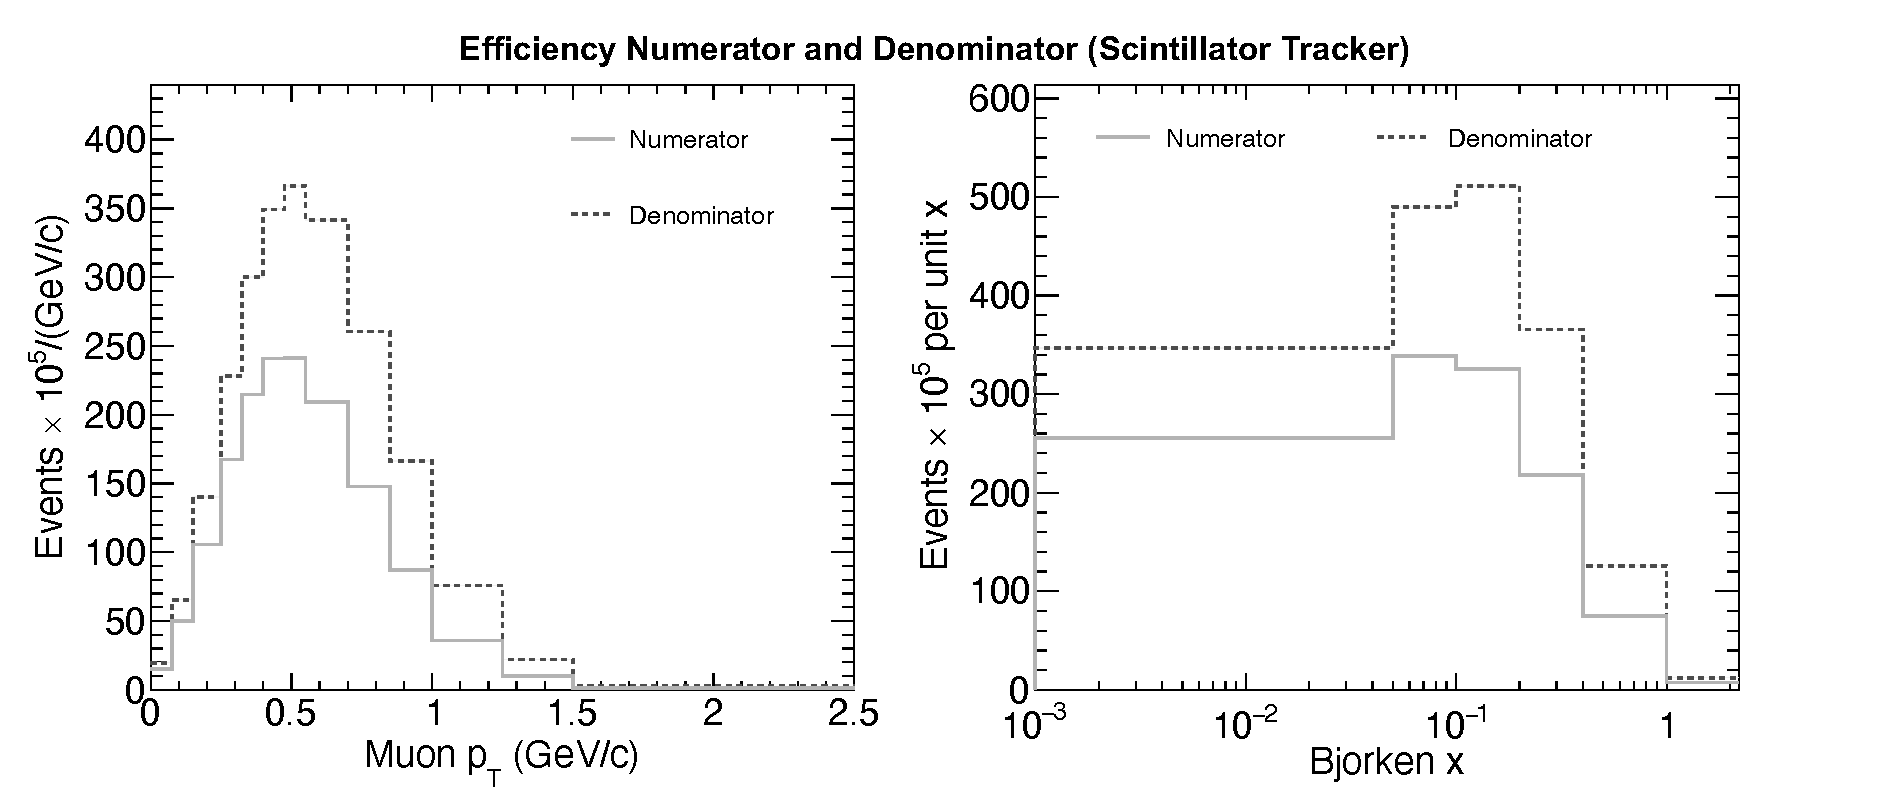
\includegraphics[width=1\textwidth]{07analysis1D/figures/efficiency_trackerNumDenom_pTx.pdf}}%
    \caption{Efficiency numerator and denominator distributions for the scintillator tracker in both $p_{\text{T}}$ (left) and Bjorken $x$ (right). The solid line for the numerator represents the generated and reconstructed signal events, while the dashed line for the denominator denotes the superset of all generated signal events.}
    %[short caption] {long caption}
    \label{fig:efficiencyNumDenom_scintillatorTracker_pTx}
\end{figure}

In practice, this means filling two histograms representing the numerator and the denominator in Equation~\ref{eq:efficiency} using the true information of the events and taking their ratio. An example of these two histograms used in the calculation of the scintillator tracker efficiency for both $p_{\text{T}}$ and Bjorken $x$ is shown in Figure \ref{fig:efficiencyNumDenom_scintillatorTracker_pTx}. While the numerator events are selected from the subsample of the reconstructed events and hence carry the systematic uncertainties associated with the detector's acceptance and event reconstruction, the denominator events are independent of them. This is demonstrated in Figure \ref{fig:efficiencyNumDenom_fracUnc} showing the systematic uncertainties of both the efficiency numerator and the denominator for the scintillator tracker as a function of $p_{\text{T}}$. 


\begin{figure}[b!]
    \centering
    {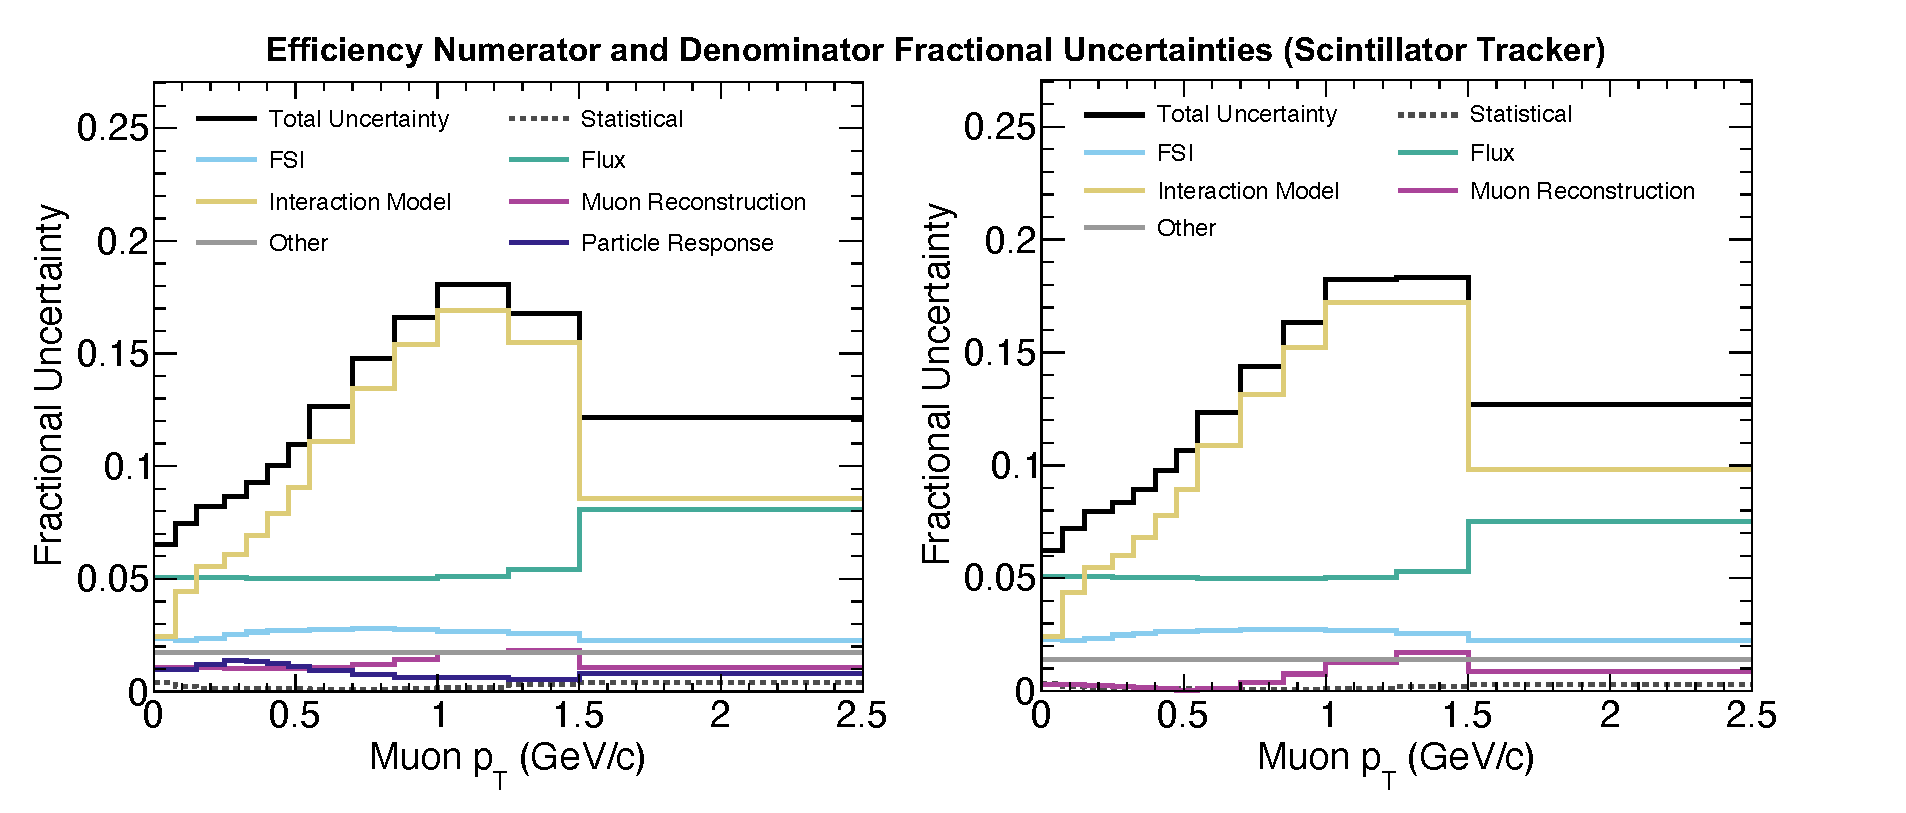
\includegraphics[width=1\textwidth]{07analysis1D/figures/efficiency_trackerNumDenomFracUnc_pT.pdf}}%
    \caption{Fractional uncertainty breakdown for the efficiency numerator (left) and the denominator (right) distributions of scintillator tracker as a function of $p_{\text{T}}$. Note the omitted `Particle Response' uncertainty band and the reduced `Muon Reconstruction' uncertainty band in the denominator uncertainty on the right.  }
    %[short caption] {long caption}
    \label{fig:efficiencyNumDenom_fracUnc}
\end{figure}

Specifically, Figure \ref{fig:efficiencyNumDenom_fracUnc} highlights that the denominator fractional uncertainty does not include the uncertainty linked to the calorimetric energy response of the detector and interaction cross-sections of particles traversing through the detector, represented by the `Particle Response' uncertainty band. The `Muon Reconstruction' uncertainty band omits all uncertainty sources except for those related to the MINOS antimuon momentum universes, which are directly correlated with flux. Finally, the `Other' uncertainty band is reduced by excluding the uncertainty associated with vertex reconstruction. A detailed description of the various systematic uncertainty bands can be found in Chapter~\ref{ch:systematics}.
%  The flux is different in the MINOS-muon-momentum-shifted universes, which means it should have an effect anywhere the Flux universes have an effect. 

\begin{figure}[b!]
    \centering
    {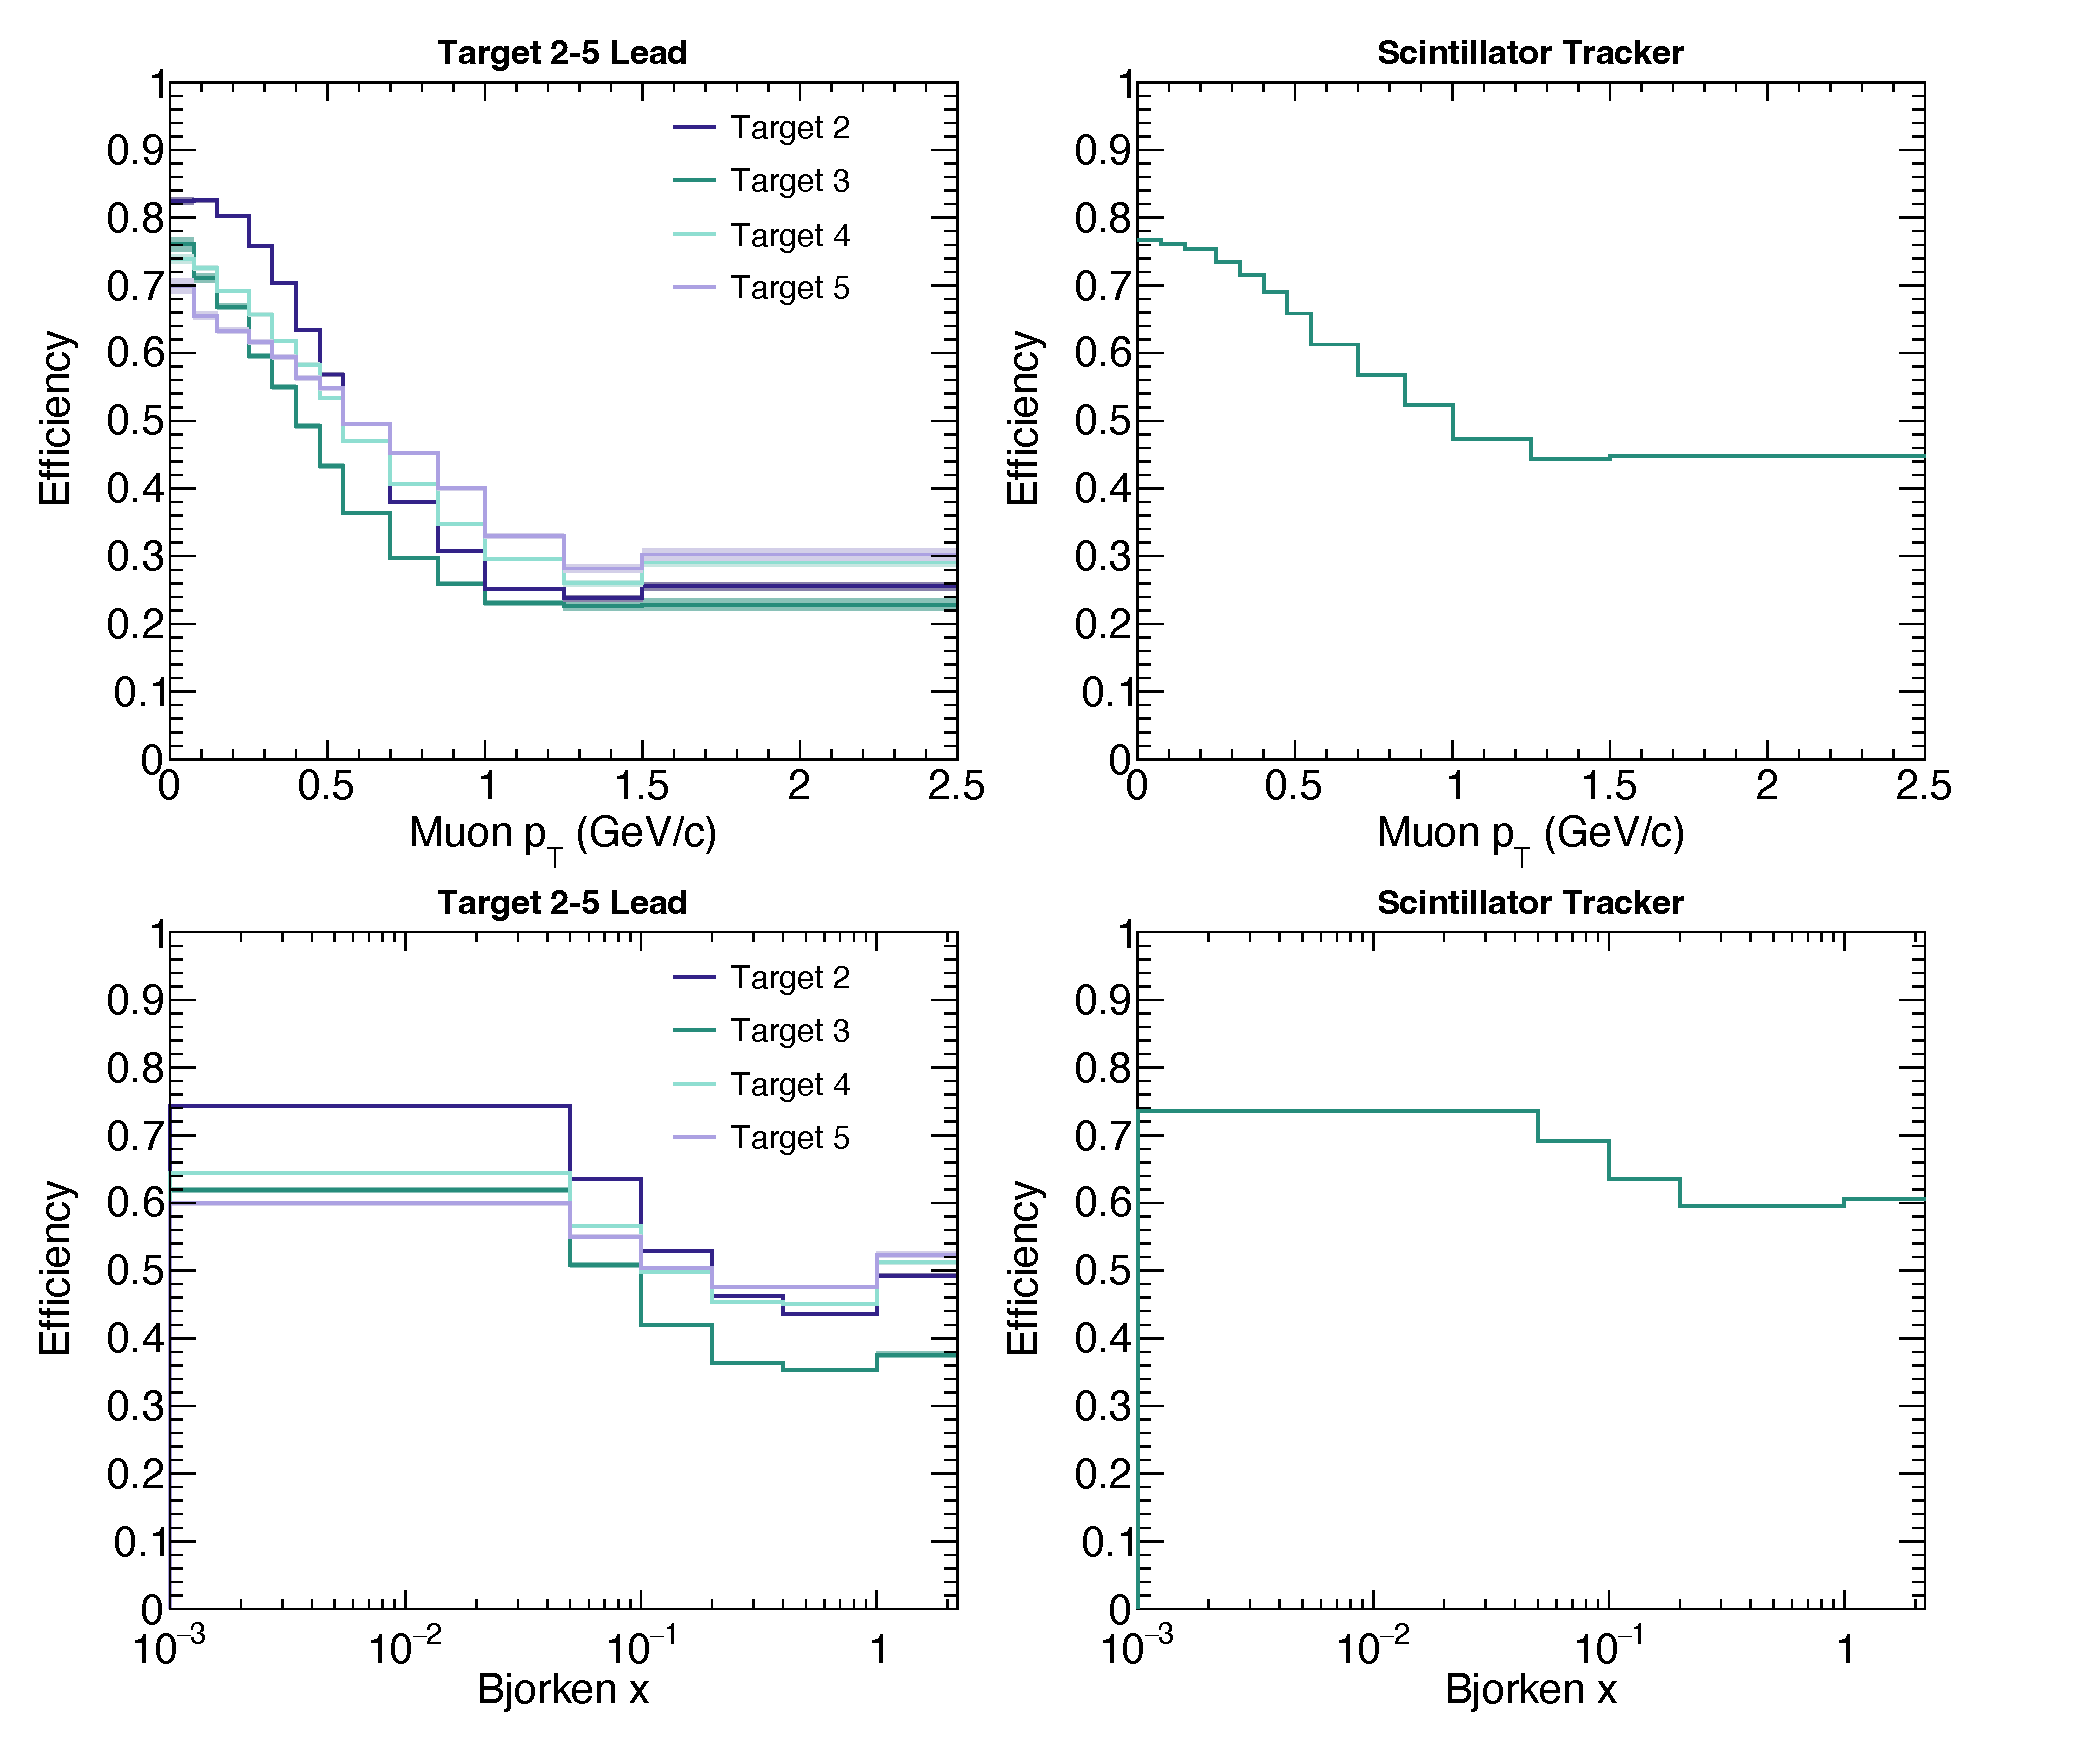
\includegraphics[width=1\textwidth]{07analysis1D/figures/efficiency_lead_tracker_pTx.pdf}}%
    \caption{Efficiency correction distributions for the various lead targets (left panel) and the scintillator tracker (right panel) as a function of $p_{\text{T}}$ (top) and Bjorken $x$ (bottom).}
    %[short caption] {long caption}
    \label{fig:efficiency_lead_tracker_pTx}
\end{figure}

Because the numerator distribution of the selected reconstructed events is a subsample of the denominator distribution of the selected generated events, the two distributions are correlated and so are their systematic uncertainties, as indicated by Figure \ref{fig:efficiencyNumDenom_fracUnc}. Consequently, when calculating the ratio, the correlations between the uncertainties are taken into account by using binomial error propagation. The efficiencies for different lead targets and the scintillator tracker both in $p_{\text{T}}$ and Bjorken $x$ are shown in Figure \ref {fig:efficiency_lead_tracker_pTx}. 

% Binomial error
% fSumw2.fArray[bin] = TMath::Abs( ( (1-2*w)*e1*e1 + w*w*e2*e2 )/(b2*b2) );  
% where w = b1/b2

Due to the inclusive nature of the analysis, the efficiency relies on detecting and reconstructing the antimuon both in the MINERvA detector and the MINOS spectrometer. The top panel of Figure \ref{fig:efficiency_lead_tracker_pTx} illustrates the fall-off in the $p_{\text{T}}$ efficiency at higher $p_{\text{T}}$. This is attributed to the fact that $p_{\text{T}}$ serves as a proxy for the antimuon angle, whose detection is constrained by the limited antimuon acceptance of the MINOS spectrometer at higher angles. Furthermore, the differences between the various lead target efficiencies in Figure~\ref{fig:efficiency_lead_tracker_pTx} can be explained due to their positions in the detector with respect to the MINOS spectrometer.

For example, target 2 lead is more upstream than target 5 lead. At lower $p_{\text{T}}$ (antimuon angle), the antimuon is likely to be more energetic than at higher $p_{\text{T}}$. This means that a~more energetic antimuon produced by an interaction in target 2 lead has to traverse more material before reaching the MINOS spectrometer and loses more energy compared to one produced in target 5 lead. Therefore, the antimuon from target 2 lead is more likely to be able to stop in the MINOS spectrometer and be reconstructed, resulting in target 2 lead having higher $p_{\text{T}}$ efficiency than target 5 lead. Conversely, an antimuon produced with a higher angle in a target more downstream and thus closer to the MINOS spectrometer is more likely to be reconstructed. This leads to target 5 lead having a~larger efficiency at higher $p_{\text{T}}$ compared to target 2 lead.

The Bjorken $x$ efficiency in the bottom panel of Figure~\ref{fig:efficiency_lead_tracker_pTx} exhibits similar behaviour as $p_{\text{T}}$. Nevertheless, the decline at higher Bjorken $x$ is less pronounced due to the weaker dependence on the antimuon angle. 

\begin{table}[b!]
    \centering

    \begin{tabular}{c c c}
    \hline \\ [-1.5 ex]
    Target & Material & Efficiency (\%) \\ [0.5ex] % inserts table %heading
    \hline
    \hline
    2 & Iron & 41.9 \\
      & Lead & 49.5 \\
    \hline
    3 & Carbon & 52.4 \\
      & Iron & 40.3 \\
      & Lead & 39.7 \\
    \hline
    4 & Lead & 47.8 \\
    \hline
    5 & Iron & 50.5\\
      & Lead & 48.8 \\
    \hline
    Tracker & Scintillator & 63.3 \\
    \hline
    \end{tabular}

    \caption{Integrated efficiency correction for all targets of different materials and the scintillator tracker.}
    \label{table:efficiency}
\end{table}


The integrated efficiency for all the targets of different materials and the scintillator tracker can be found in Table~\ref{table:efficiency}. For targets in particular, the efficiency depends on the ability to reconstruct the vertex in the nuclear target, as detailed in Chapter~\ref{ch:Reconstruction}. Furthermore, within a given target, the efficiency is lower for materials that shadow the MINOS coil described in Chapter~\ref{ch:minerva}, such as iron in the second target or lead in the fifth target.

\begin{figure}[b!] 
    \centering
    {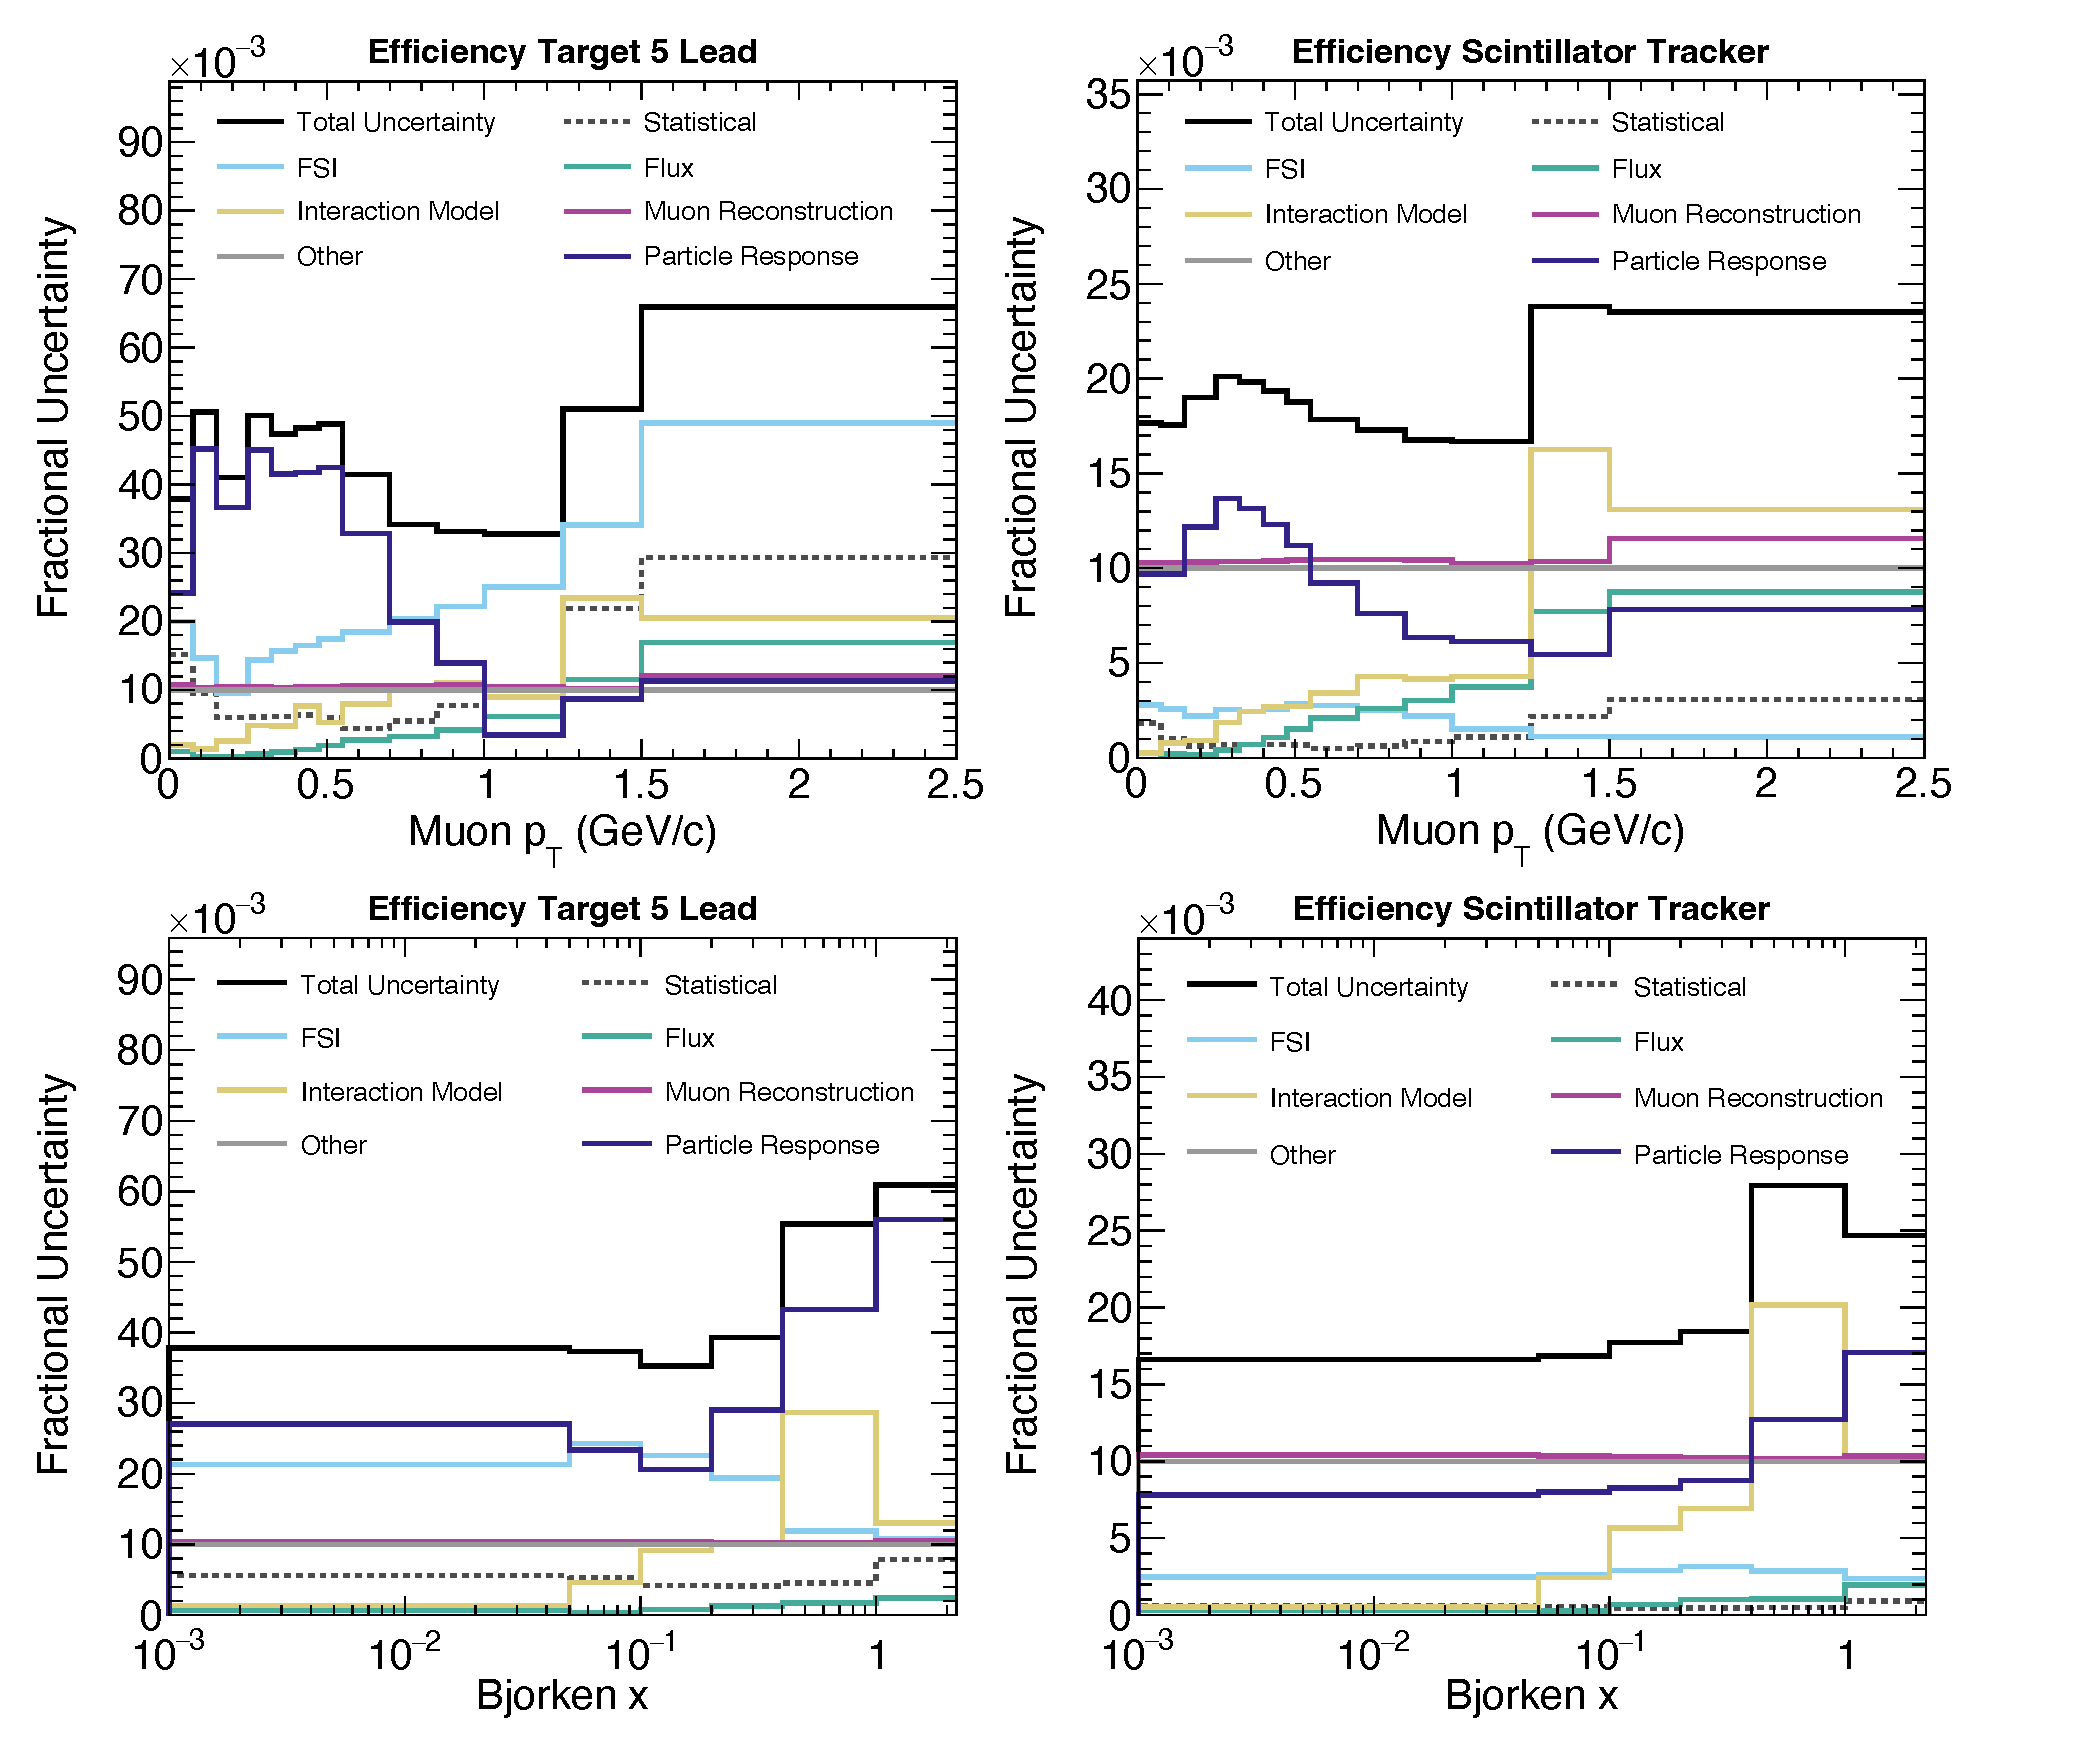
\includegraphics[width=1\textwidth]{07analysis1D/figures/efficiency_lead_tracker_pTx_fracErr.pdf}}%
    \caption{Fractional uncertainty breakdown for the efficiency of target 5 lead (left panel) and scintillator tracker (right panel) as a function of $p_{\text{T}}$ (top) and Bjorken $x$ (bottom). Note the increase in the `FSI' uncertainty band for lead compared to the scintillator. }
    %[short caption] {long caption}
    \label{fig:efficiency_lead_tracker_pTx_fracErr}
\end{figure}

% systematics
The fractional uncertainty on the target 5 lead and scintillator tracker efficiency in both $p_{\text{T}}$ and Bjorken $x$ is shown in Figure~\ref{fig:efficiency_lead_tracker_pTx_fracErr}. The region of low $p_{\text{T}}$ and high Bjorken~$x$, mainly associated with quasi-elastic events, is dominated by the `Particle Response' uncertainty coming from the efficiency numerator. Specifically, this uncertainty is mostly attributed to the uncertainty on the neutron cross-section. Additionally, both high $p_{\text{T}}$ and high Bjorken~$x$ have prominent `Interaction Model' uncertainty bands, primarily arising from the resonance production model. Figure~\ref{fig:efficiency_lead_tracker_pTx_fracErr} also illustrates that the `FSI' uncertainty band is more pronounced the heavier the nucleus is, i.e. heavy lead versus relatively light scintillator in comparison. The `FSI' band is overall governed by the pion absorption cross-section uncertainty. 


\begin{figure}[t!] 
    \centering
    {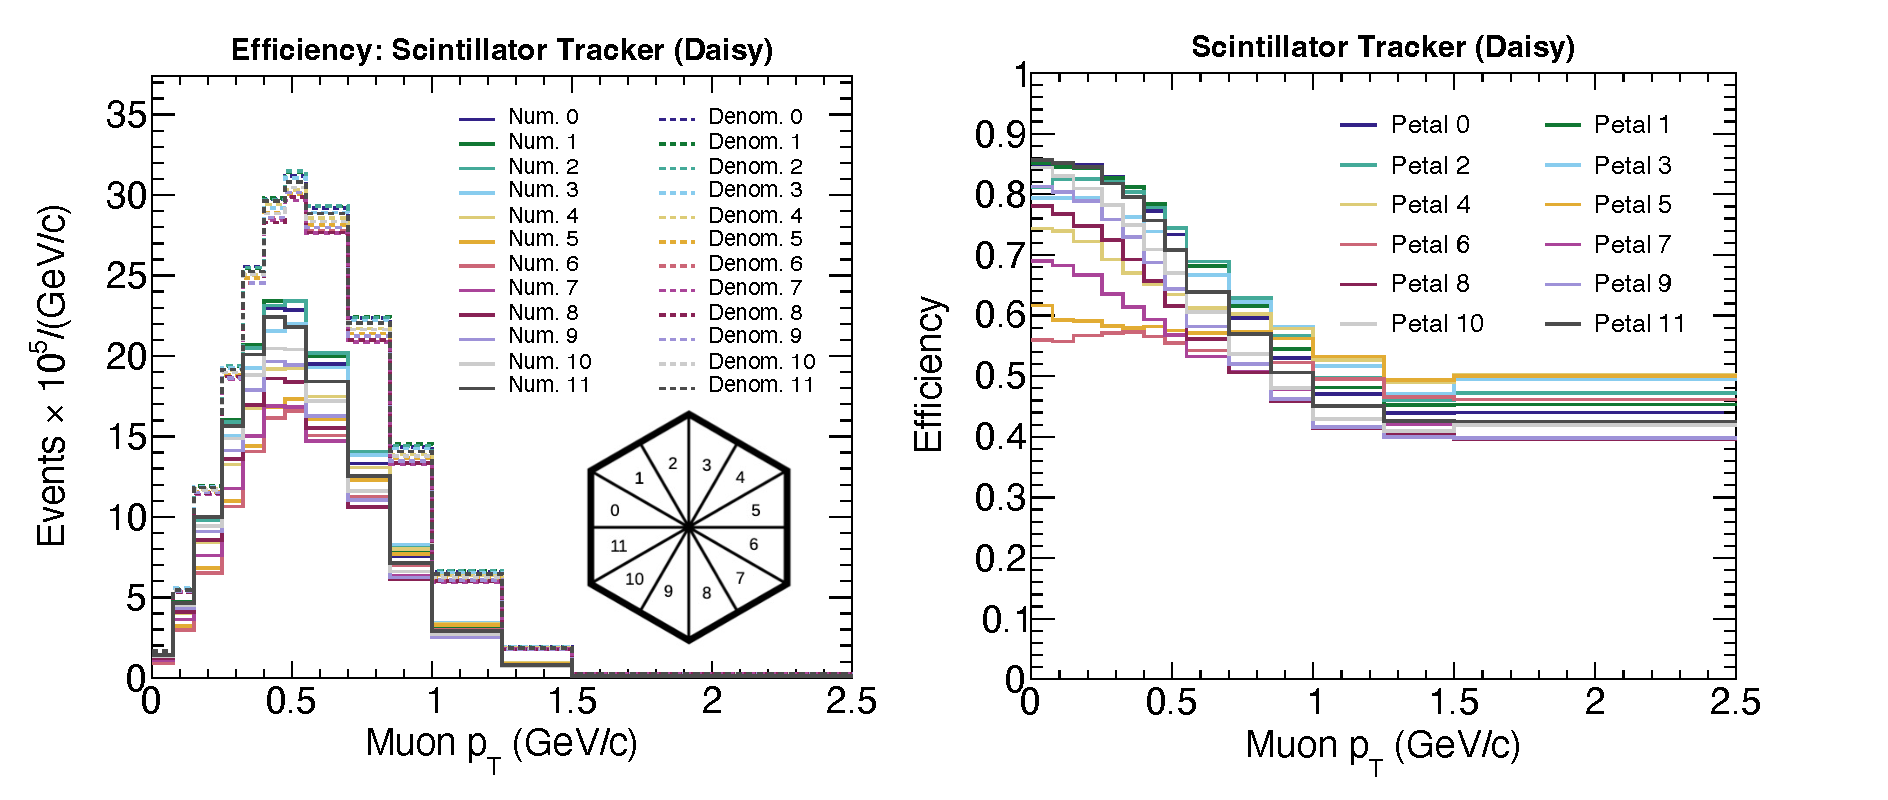
\includegraphics[width=1\textwidth]{07analysis1D/figures/efficiency_tracker_pT_daisy.pdf}}%
    \caption{Left:~Efficiency numerator and denominator for the scintillator tracker in `daisy petals' in antimuon $p_{\text{T}}$.~The hexagon insert illustrates petal positions looking downstream of the detector.~Right:~Efficiency distribution for the scintillator tracker in `daisy petals' in antimuon $p_{\text{T}}$. }
    %[short caption] {long caption}
    \label{fig:efficiency_tracker_pT_daisy}
\end{figure}


Finally, it is important to note that the scintillator tracker efficiency is also extracted in the `daisy petals', as illustrated in Figure~\ref{fig:efficiency_tracker_pT_daisy} for $p_{\text{T}}$. This extraction is essential for determining nuclear target-to-scintillator cross-section ratios using the matching flux technique discussed in Section~\ref{sec:nuclear_target_flux}. Similarly to the passive targets, the petals shadowing the MINOS coil have reduced efficiency at low $p_{\text{T}}$. All efficiency correction distributions for passive targets, scintillator tracker, and scintillator tracker divided in the `daisy petals' and their corresponding fractional uncertainties are included in Appendix~\ref{ch:appendix_efficiencyCorrection}.


\begin{comment}
After the efficiency correction, individual targets of the same material can be combined. In practice, this means adding up the efficiency-corrected histograms for targets 2,3 and 5 iron and 2-5 lead. Furthermore, the individual `daisy petals' of the scintillator tracker can be combined for cross-section ratios - a linear combination of the 

An example of the lead efficiency-corrected distribution, its fractional uncertainty and the scintillator tracker combined to match the individual targets is shown. The fractional error on the base scintillator tracker unfolded distributions is shown for comparison. 
\end{comment}

[Plots of efficiency-corrected distributions]

[For tracker cross-section used in cross-section ratios, this is where the individual distributions get combined]

\newpage
\section{Normalisation}

The final step in the calculation of the differential cross-section involves normalising the efficiency-corrected distribution according to the Equation~\ref{eq:xsec1D}.~First, each bin of the
efficiency-corrected distribution is divided by the number of scattering centres $T_{\text{nucleons}}$, i.e. the number of nucleons, within the fiducial volume available for an antineutrino to interact with in a given material.~Reporting the cross-section per nucleon ensures the result is independent of the detector's mass. The estimates of the number of nucleons in Table~\ref{table:normalisation} are derived from MINERvA's material assays~\cite{Aliaga_2014}. 

Furthermore, to report a differential cross-section, one must divide each bin $\alpha$ of the efficiency-corrected distribution by the integrated antineutrino flux prediction $\Phi$ and the corresponding bin width $\Delta x_{\alpha}$.~The antineutrino flux integral is calculated as a function of true antineutrino energy between 0--120~GeV using the flux simulation prediction outlined in Sections~\ref{sec:NuMI} and \ref{sec:fluxSimulation}.~The upper limit is determined by the 120~GeV/$c$ protons from which the NuMI antineutrino beam originates.~However, the contribution above 20~GeV is negligible as illustrated in Figure \ref{fig:antinu_fluxes} due to the muon energy cut discussed in Section~\ref{sec:eventSelection}. 

In line with the discussion in Section~\ref{sec:nuclear_target_flux}, Figure \ref{fig:antinu_fluxes} illustrates that antineutrino fluxes across different materials vary.~Consequently, the antineutrino flux integrals per protons on target (POT) are also shown to vary for different materials in Table~\ref{table:normalisation}. To eliminate the POT dependence, each flux integral in Table \ref{table:normalisation} is multiplied by the total data exposure of $1.12 \times 10^{21}$ POT in the cross-section extraction. A simple dimensional analysis shows that the differential cross-sections $\text{d}\sigma/\text{d}p_{T}$ and $\text{d}\sigma/\text{d}x$ can be reported in units of $10^{-39}/\text{cm}^{2}/\text{unit}/\text{nucleon}$, where `unit' represents the unit of the kinematic variable for which the differential cross-section was calculated.


%The flux normalisation also propagates the uncertainties associated with the flux, which are explained in Chapter~\ref{ch:systematics}.

%while accounting for the uncertainty associated with the target masses described in Chapter~\ref{ch:systematics}.
%N neutrons: mass * TargetProp::AtomsPerGram::C   * TargetProp::NeutronsPerAtom::C;

\begin{figure}[t!] 
    \centering
    {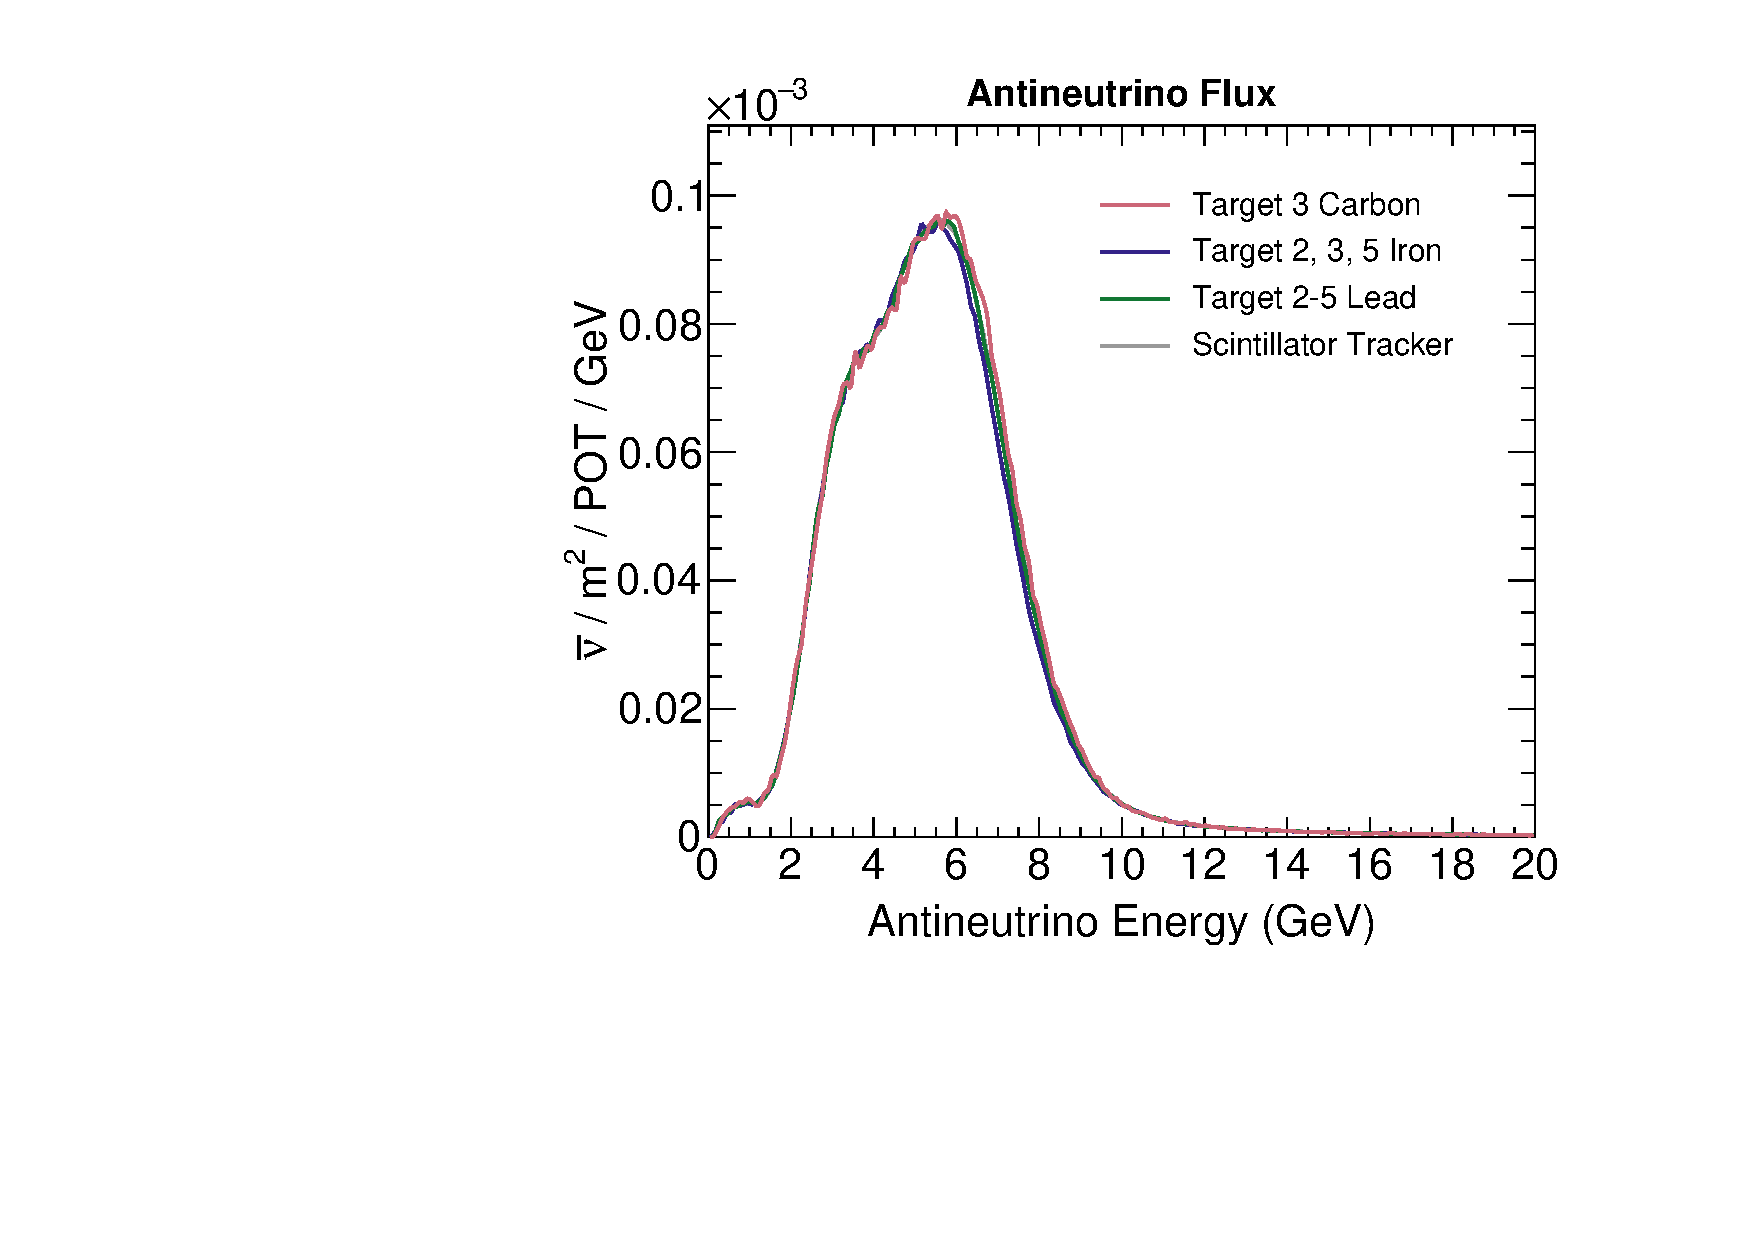
\includegraphics[width=1\textwidth]{07analysis1D/figures/antinu_flux.pdf}}%
    \caption{Antineutrino flux as a function of antineutrino energy between 0--20~GeV for carbon, iron, lead, and scintillator tracker. The contribution above 20~GeV is negligible.}
    %[short caption] {long caption}
    \label{fig:antinu_fluxes}
\end{figure}



\begin{table}[b!]
    \centering

    \begin{tabular}{c c c}
    \hline \\ [-1.5 ex]
    Material & $\Phi$ $(\bar{\nu}_{\mu} \times 10^{-8}/\text{cm}^{2}/\text{POT})$ & $T_{\text{nucleons}}$ $(\times 10^{28})$ \\ [0.5ex] % inserts table %heading
    \hline\hline
    Carbon & 4.853 & 9.598 \\ %9.59755e+28 \\
    %\hline
    Iron & 4.676 & 37.841 \\ % 3.78413e+29 \\
    %\hline
    Lead & 4.763 & 42.768 \\%4.27675e+29 \\
    %\hline
    Scintillator & 4.774 & 323.478 \\ %3.23478e+30 \\
    \hline
    \end{tabular}

    \caption{Cross-section normalisation factors for the passive target region and the scintillator tracker.}
    \label{table:normalisation}
\end{table}


\section{Cross-section distributions}
\section{Cross-section ratios}
\section{Validation}


